\documentclass[preprint,12pt]{elsarticle}
\usepackage[utf8]{inputenc}
\DeclareUnicodeCharacter{0394}{\ensuremath{\Delta}}
\DeclareUnicodeCharacter{00B1}{\ensuremath{\pm}}
\DeclareUnicodeCharacter{03B1}{\ensuremath{\alpha}}
\DeclareUnicodeCharacter{03B2}{\ensuremath{\beta}}
\usepackage{amsmath,amssymb,amsfonts}
\usepackage{algorithmic}
\usepackage{graphicx}
\usepackage{textcomp}
\usepackage{booktabs}
\usepackage{multirow}
\usepackage{array}
\usepackage{url}
\usepackage{hyperref}
\usepackage{microtype}
\usepackage{xcolor}
\usepackage{lineno}

\hypersetup{
    colorlinks=true,
    linkcolor=blue,
    citecolor=blue,
    urlcolor=blue
}

\journal{Computers in Biology and Medicine}

\begin{document}

\begin{frontmatter}

\title{Positive-Class Weighting Induces Systematic Probability Distortion in Deep Learning Models for Chest Radiography under Deidentified-Date Cohort Shift}

\author{Vishesh Panghal\corref{cor1}}
\ead{pvt.panghal@gmail.com}
\cortext[cor1]{Corresponding author.}

\affiliation{organization={Department of Artificial Intelligence and Data Science, Poornima Institute of Engineering and Technology (PIET)},
            city={Jaipur},
            postcode={302022},
            state={Rajasthan},
            country={India}}

\begin{abstract}
Clinical deep learning models frequently exhibit calibration decay under deidentified-date cohort shift. Under extreme class imbalance, training with positive-weighted binary cross-entropy (BCE) is standard practice, but its downstream effect on probability calibration has been widely conflated with intrinsic feature drift. We resolve this conflation through a controlled $2 \times 2$ experimental design comprising two architectures and two loss objectives, with three independently trained random seeds per configuration (12 models total) on 40,523 chest radiographs from BRAX. Models are trained on an anchor partition and evaluated across later deidentified-date strata ($T_1, T_2, T_3$) with strict patient isolation. We show that positive loss weighting mathematically induces an additive population logit shift of $\log w$, which temperature scaling structurally cannot correct. In finite networks, empirical logit differences cluster tightly around theoretical $\log w$ (mean $\Delta z = 3.29 \pm 0.81$ vs. theoretical $3.07$ for Pleural Effusion). On stratum $T_3$, zero-parameter analytic offset ($z - \log w$) reduces total Brier score by 74\% ($\Delta\text{Brier} = -0.0795$ [95\% CI: $-0.0893, -0.0697$]), substantially reducing intercept miscalibration from $\alpha = -2.96$ to $-0.45$ without retraining or validation data. On an external MIMIC-CXR-JPG cohort (3,403 radiographs, 289 patients), discrimination proved pathology-dependent (Pleural Effusion AUROC $0.688$; Cardiomegaly $0.523$), with severe baseline calibration shift ($\text{BSS} < 0$). Analytic offset yielded significant Brier reductions for Cardiomegaly and Pneumonia, but worsened Edema, delineating boundaries of zero-parameter recalibration under cross-institutional shift. Finally, selective prediction simulations expose operational trade-offs between risk estimation and high-sensitivity screening triage.
\end{abstract}

\begin{keyword}
Chest radiography \sep Probability calibration \sep Class imbalance \sep Distribution shift \sep Selective prediction \sep Deep learning \sep Clinical decision support
\end{keyword}

\begin{highlights}
\item Positive loss weighting induces an additive population logit offset of $\log w$.
\item Finite neural network logits empirically cluster tightly around theoretical $\log w$.
\item Temperature scaling cannot correct this intercept-type calibration bias.
\item Analytic offset ($z - \log w$) cuts 74\% of Brier error without retraining.
\item Selective triage exposes trade-offs between calibrated risk and screening referral.
\end{highlights}

\begin{graphicalabstract}
\centering
\vspace*{\fill}
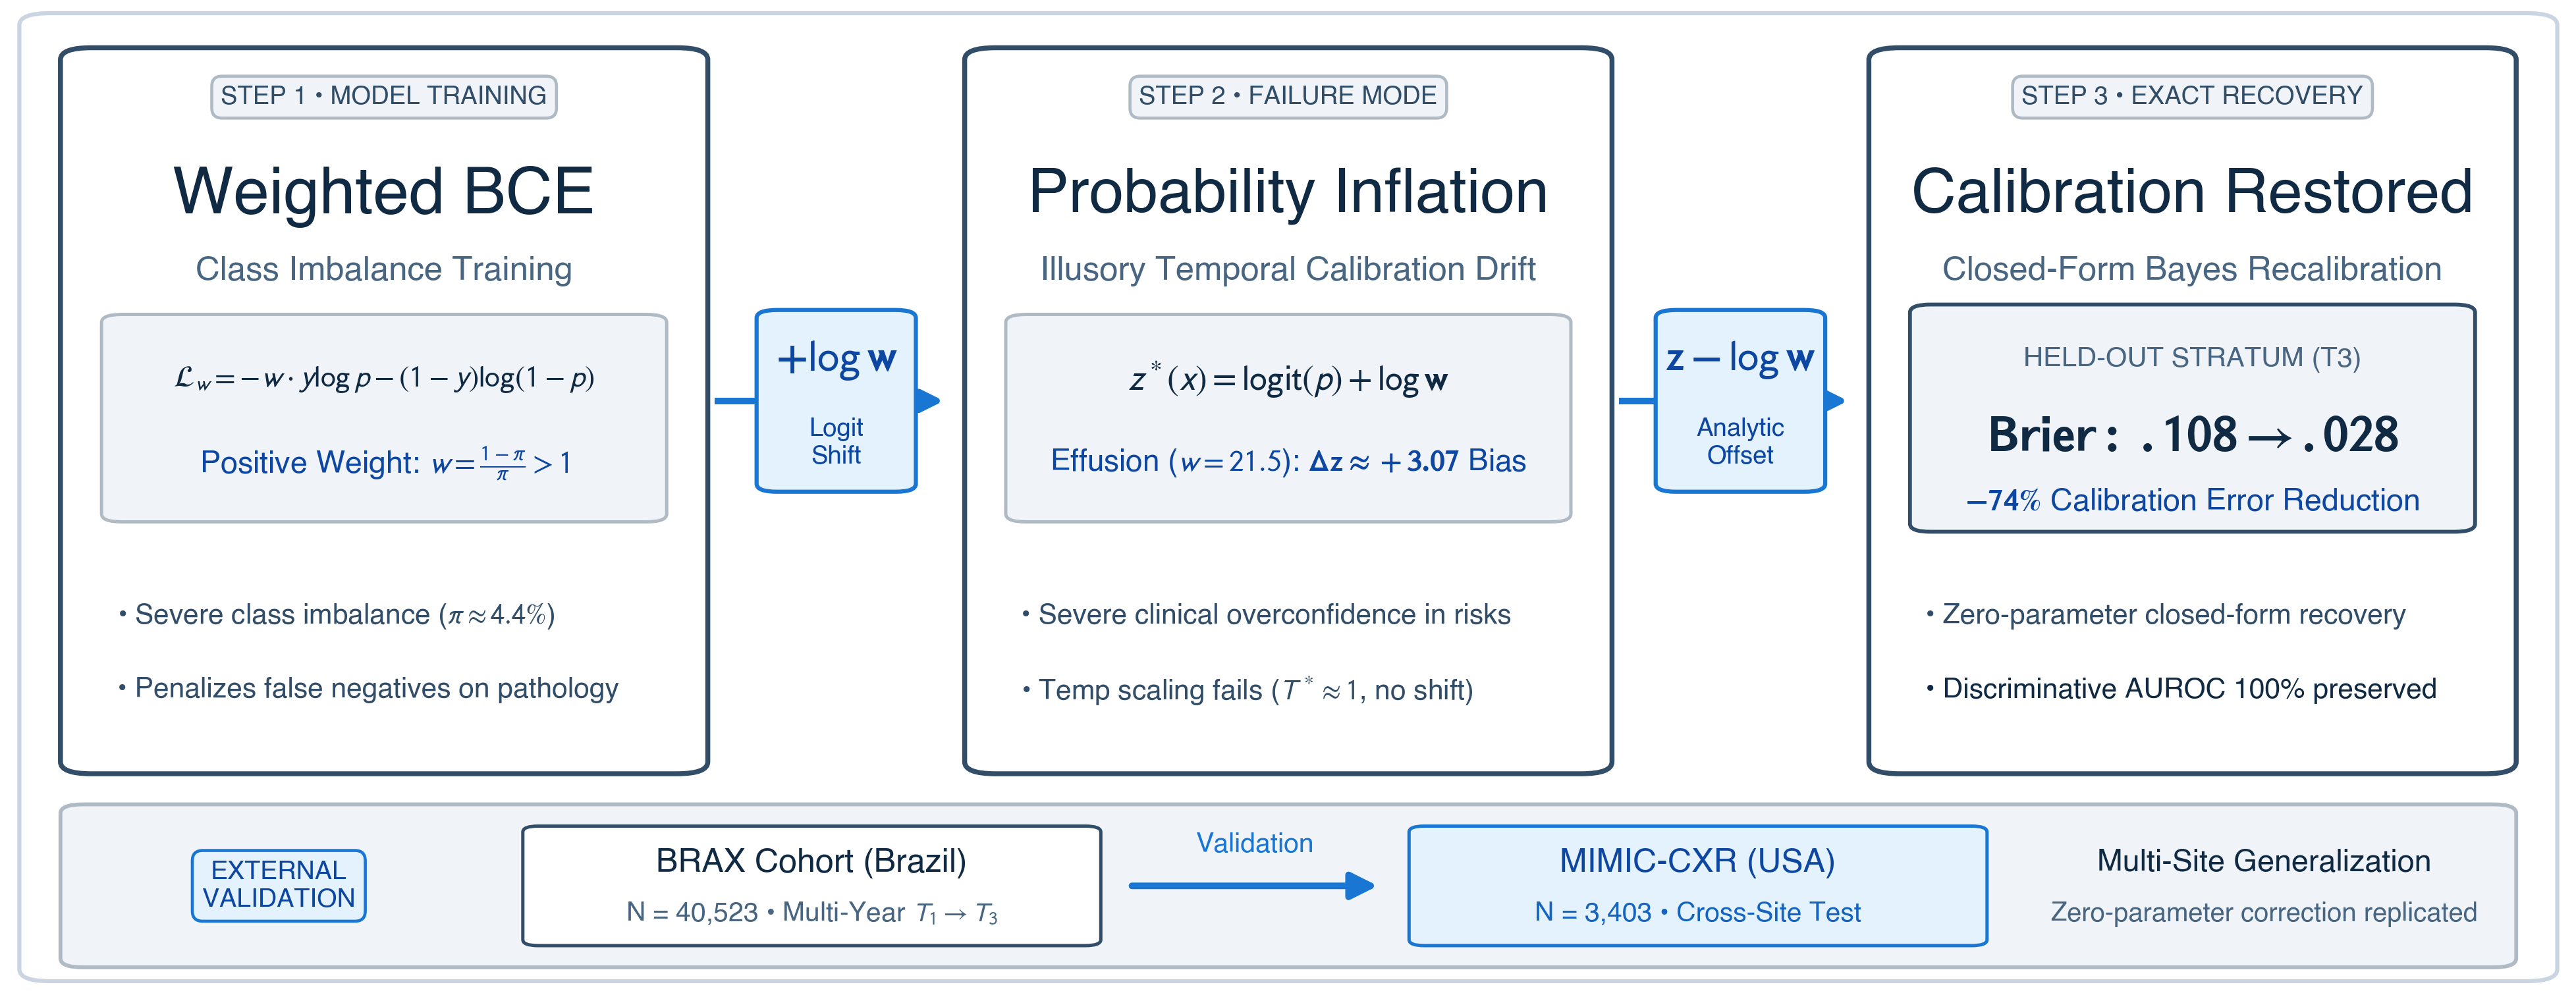
\includegraphics[width=\textwidth]{graphical_abstract.png}
\vspace*{\fill}
\end{graphicalabstract}

\end{frontmatter}

\linenumbers

\section{Introduction}
Deep learning models for automated chest radiograph interpretation have achieved high discriminatory performance across common thoracic abnormalities such as pleural effusion, cardiomegaly, and pneumonia~\cite{rajpurkar2017chexnet, reis2022brax}. However, the transition from stationary retrospective validation to longitudinal clinical deployment introduces substantial distribution shifts. In operational healthcare environments, patient populations evolve, imaging protocols shift, scanner hardware is replaced, and demographic or seasonal patterns alter condition prevalence over time~\cite{finlayson2021clinician, kore2024empirical, shenouda2023assessment}.

While discriminatory ranking (measured via AUROC) often exhibits gradual longitudinal attenuation under temporal shift, decision-critical applications rely fundamentally on \textit{calibrated posterior probabilities}: $P(Y = 1 \mid X = x)$~\cite{vancalster2019calibration, steyerberg2010assessing}. When predicted probabilities deviate from true empirical event rates, downstream operational decision cutoffs shift unpredictably, expected utility formulations degrade, and automated decision-support pipelines generate distorted risk rankings.

Recent literature has reported rapid ``temporal calibration decay,'' asserting that frozen deep neural networks suffer progressive miscalibration over deployment periods~\cite{guo2022evaluation, hinson2022multisite}. Simultaneously, because biomedical datasets are characterized by extreme class imbalance (pathology prevalence often below 5\%), researchers routinely train vision models using positive-weighted binary cross-entropy (BCE) to penalize missed positive cases~\cite{rajpurkar2017chexnet, buda2018systematic}. 

In this work, we present a computational investigation showing that these two phenomena are deeply entangled, and that the prevailing attribution of temporal calibration degradation primarily to intrinsic feature drift may be largely explained by uncorrected post-training calibration offsets under label distribution shifts~\cite{alexandari2020maximum, davis2020detection}. Under population-risk minimization, when models are trained with positive loss weighting $w > 1$, the Bayes-optimal logit is shifted by an additive constant $+\log w$~\cite{king2001logistic, caplin2022calibrating}. In theoretical machine learning, Caplin, Martin, and Marx~\cite{caplin2022calibrating} formally established that class weighting is fundamentally incompatible with unadjusted probability calibration and derived an inverse machine learning formulation to recover true likelihoods, demonstrating this on a static chest radiograph pneumonia task. Standard post-hoc calibration methods---most notably temperature scaling~\cite{guo2017calibration}---only rescale the logit variance ($z / T$) and cannot shift the logit intercept. Consequently, weighted models continuously over-predict positive probabilities, producing severe Brier score and Expected Calibration Error (ECE) degradation that compounds over time as disease prevalence fluctuates.

\subsection{Related Work}
\textbf{Probability Calibration in Deep Learning:} Modern deep convolutional neural networks frequently exhibit over-confidence due to unconstrained cross-entropy minimization with over-parameterized architectures~\cite{guo2017calibration}. Post-hoc recalibration techniques such as temperature scaling, histogram binning, and isotonic regression have been widely evaluated~\cite{guo2017calibration, platt1999probabilistic}. In medical decision models, calibration accuracy is paramount for valid risk stratification~\cite{vancalster2019calibration, steyerberg2010assessing}. However, standard methods were primarily derived for multi-class classification under balanced distributions, leaving binary imbalanced settings less formally explored.

\textbf{Class Imbalance and Loss Function Design:} Extreme class imbalance is pervasive in thoracic imaging. Common mitigation strategies include positive loss weighting~\cite{buda2018systematic, rajpurkar2017chexnet}, focal loss~\cite{lin2017focal}, and re-sampling. In clinical prediction modeling, Piccininni et al.~\cite{piccininni2024understanding} formally demonstrated that correcting class imbalance through resampling inherently alters the effective sampling proportion and damages probability calibration, while showing that plug-in probability corrections can recover valid absolute risks while discrimination remains largely preserved. In loss-based weighting, King and Zeng~\cite{king2001logistic} established in classical logistic regression that choice-based sample proportion adjustments induce an intercept shift of $\log w$. More recently, Caplin, Martin, and Marx~\cite{caplin2022calibrating} analyzed loss-weighted deep learning through an economic modeling lens, rigorously establishing that class weighting is mathematically incompatible with raw posterior probability calibration. They formulated an inverse machine learning framework to recover undistorted likelihoods from weighted models and demonstrated feasibility on a static CheXNet pneumonia detection task~\cite{rajpurkar2017chexnet}. However, their work was confined to stationary single-dataset evaluations, leaving unexamined how loss-induced logit shifts behave under sequential temporal cohort shifts, whether standard deep calibration methods (temperature scaling) fail under this distortion, how finite neural networks optimize under extreme class scarcity, and how post-hoc recalibration behaves under cross-institutional transfer. Modern clinical pipelines routinely deploy weighted architectures without correcting for this induced logit offset prior to post-hoc calibration.

\textbf{Distribution Shift and Label Shift Adaptation:} Temporal dataset shift encompasses changes in feature distributions $P(X)$, conditional distributions $P(Y \mid X)$, and prior label probabilities $P(Y)$~\cite{finlayson2021clinician}. Davis et al.~\cite{davis2020detection} demonstrated that calibration drift often precedes discriminatory loss in clinical models. Alexandari et al.~\cite{alexandari2020maximum} established that maximum likelihood with bias-corrected calibration provides robust adaptation under label shift. Decoupling algorithmic training offsets from genuine temporal shift is essential for diagnostic integrity.

\textbf{Selective Prediction and Deferral Mechanisms:} Selective classification allows models to abstain from predicting on ambiguous inputs, routing them to human experts~\cite{geifman2017selective, kompa2021second}. Fisch et al.~\cite{fisch2022calibrated} highlighted that selective classification performance is fundamentally bounded by probability calibration. Recently, Aperstein et al.~\cite{aperstein2026knowing} demonstrated multi-pathology chest radiograph selective prediction across PadChest, NIH ChestX-ray14, and MIMIC-CXR using entropy- and confidence-based rejection mechanisms evaluated via risk-coverage profiles and bootstrap inference. While such studies focus on developing abstention policies, the interaction between underlying loss-induced calibration distortion and downstream selective triage remains largely unexplored. In this work, rather than proposing a new abstention algorithm, we utilize selective prediction as an operational downstream lens to evaluate the real-world clinical consequences of calibration mechanisms, exposing how loss weighting and calibration alter referral efficiency and screening recall under workflow constraints.

\subsection{Contributions}
To disentangle algorithmic loss bias from distribution shift across cohort strata, this paper provides:
\begin{enumerate}
    \item \textbf{A Controlled $2 \times 2$ Experimental Design:} We execute a controlled $2 \times 2$ experimental design comprising two architectures and two loss objectives (DenseNet-121 and ResNet-50 $\times$ standard BCE and positive-weighted BCE), with three independently trained random seeds per configuration (12 models total) trained on 25,123 chest radiographs and evaluated on 8,302 held-out radiographs across three sequential deidentified-date strata ($T_1, T_2, T_3$) from the BRAX dataset~\cite{reis2022brax}.
    \item \textbf{Theoretical Derivation and Empirical Verification of Logit Shift:} Extending foundational observations of loss-induced probability distortion~\cite{king2001logistic, caplin2022calibrating} into longitudinal clinical deep learning, we derive that positive-weighted BCE introduces a constant population logit offset $\log w$. Across 16,604 evaluations spanning two convolutional backbones and diverse thoracic pathologies, we empirically demonstrate where finite neural networks tightly adhere to theoretical $\log w$ and delineate where extreme class scarcity ($w > 1000$) causes optimization saturation. Crucially, we prove that standard temperature scaling is structurally incapable of correcting this logit intercept displacement ($\alpha \approx -2.96$), whereas an exact zero-parameter analytic offset ($z - \log w$) or non-negative Platt scaling restores calibration parity with unweighted models (substantially reducing intercept bias to $\alpha = -0.45$ for DenseNet-121 and reducing total Brier error by 74\%--76\%).
    \item \textbf{A Leak-Free Out-of-Sample Calibration Protocol:} We implement a strict 5-fold patient-clustered cross-fitting protocol on $T_1$, strictly preventing in-sample calibration leakage, and report out-of-sample generalization on $T_2$ and $T_3$ backed by 2,000-replicate patient-clustered bootstrap confidence intervals directly on individual seeds and the 3-seed ensemble.
    \item \textbf{Operational Selective Prediction and Workload Triage Analysis:} Rather than proposing an independent abstention algorithm, we utilize selective prediction as an operational downstream lens with explicit, transparent tracking of reader referral workloads, retained sensitivity ($TP / N_{\text{pos, ret}}$), and full-cohort system sensitivity ($1 - FN / N_{\text{pos, total}}$) under matched development thresholds, demonstrating that calibrated models optimize probability estimation while raw weighted models support recall-oriented screening triage.
\end{enumerate}

\section{Materials and Methods}

\subsection{Dataset and Cohort Stratification}
We utilize the Brazilian Chest X-ray (BRAX) v1.1.0 benchmark~\cite{reis2022brax}. BRAX v1.1.0 contains 40,967 radiographs. After excluding 444 radiographs from 89 patients whose examinations crossed partition boundaries, the analytic cohort comprised 40,523 radiographs acquired across multiple inpatient and outpatient emergency facilities at Hospital Israelita Albert Einstein in S\~ao Paulo, Brazil. Radiographs are labeled with 14 thoracic findings extracted from Portuguese radiological reports using a validated natural language processing pipeline.

In compliance with HIPAA de-identification standards, direct patient identifiers and original timestamps are protected. We extract chronological study dates from the released 8-digit calendar integers (\texttt{YYYYMMDD}), spanning 2008 through 2017. BRAX documentation states that the released dates are fictitious dates generated through a hashing procedure while retaining the original intervals between study acquisitions. Because synchronization of anonymized dates across different patients is not explicitly established, we interpret these partitions as sequential deidentified-date strata rather than real-world calendar periods. To maintain strict partition integrity and preclude longitudinal data leakage:
\begin{enumerate}
    \item All studies are partitioned chronologically around a strict model freeze boundary: $T_{\text{freeze}} = \text{2015-07-01}$.
    \item All training studies occur before 2013-09-01 ($N = 25,123$ images from 11,265 patients across 14,315 studies).
    \item All validation studies occur between 2013-09-01 and 2015-06-30 ($N = 7,098$ images from 3,281 patients across 4,012 studies).
    \item All held-out test studies occur between 2015-07-01 and 2017-12-17 ($N = 8,302$ images from 3,807 patients across 4,670 studies), partitioned into three consecutive deidentified-date strata: $T_1$ (2015-H2, $N=1,879$), $T_2$ (2016, $N=3,987$), and $T_3$ (2017, $N=2,436$).
    \item Strict patient isolation is enforced: $\text{Patients}_{\text{train}} \cap \text{Patients}_{\text{val}} \cap \text{Patients}_{\text{test}} = \emptyset$. Specifically, 444 radiographs from 89 patients whose examinations crossed partition boundaries were excluded to guarantee zero within-patient contamination, yielding the analytic cohort of 40,523 radiographs.
    \item For longitudinal paired logit offset and multi-calibrator evaluation, all $8,302$ held-out radiographs ($N=1,879$ in $T_1$, $N=3,987$ in $T_2$, and $N=2,436$ in $T_3$) are evaluated across both clinical architectures (DenseNet-121 and ResNet-50) with zero held-out exclusions ($0\%$ exclusion rate), yielding $16,604$ paired ensemble evaluations ($8,302 \times 2$ image-architecture pairs with 3 seed replications averaged per pair; $49,812$ total seed-level pairs) with complete longitudinal tracking.
\end{enumerate}

Demographic, projection, and disease prevalence characteristics across all cohort strata are detailed in Table~\ref{tab:cohort_demographics}.

\begin{table*}[!t]
\caption{Cohort Demographics, Radiographic Projections, and Target Condition Prevalence across Stratified Cohorts}
\label{tab:cohort_demographics}
\centering
\resizebox{\textwidth}{!}{%
\begin{tabular}{lllllllllll}
\toprule
Cohort Stratum & Images (N) & Patients (N) & Studies (N) & Sex (\% M / F) & Age (Mean ± SD) & Views (\% PA / AP / Lat / Unk) & Pleural Effusion N (\%) & Cardiomegaly N (\%) & Pneumonia N (\%) & Edema N (\%) \\
\midrule
Train (Pre-deployment) & 25,123 & 11,265 & 14,315 & 49.3\% / 50.7\% & 46.0 ± 24.3 & 34.0\% / 13.5\% / 0.0\% / 27.2\% & 1,116 (4.44\%) & 2,398 (9.55\%) & 456 (1.82\%) & 23 (0.09\%) \\
Val (Pre-deployment) & 7,098 & 3,281 & 4,012 & 49.8\% / 50.2\% & 46.2 ± 24.1 & 34.7\% / 12.2\% / 0.0\% / 27.7\% & 295 (4.16\%) & 681 (9.59\%) & 128 (1.80\%) & 8 (0.11\%) \\
Test T1 (2015) & 1,879 & 913 & 1,039 & 47.8\% / 52.2\% & 44.5 ± 23.9 & 34.4\% / 10.2\% / 0.0\% / 29.0\% & 99 (5.27\%) & 147 (7.82\%) & 50 (2.66\%) & 4 (0.21\%) \\
Test T2 (2016) & 3,987 & 1,832 & 2,249 & 48.5\% / 51.5\% & 46.1 ± 23.8 & 34.6\% / 12.0\% / 0.0\% / 27.6\% & 177 (4.44\%) & 422 (10.58\%) & 79 (1.98\%) & 13 (0.33\%) \\
Test T3 (2017) & 2,436 & 1,164 & 1,382 & 50.9\% / 49.1\% & 46.0 ± 24.6 & 34.4\% / 12.4\% / 0.0\% / 28.1\% & 85 (3.49\%) & 258 (10.59\%) & 50 (2.05\%) & 0 (0.00\%) \\
Test All (Pooled) & 8,302 & 3,807 & 4,670 & 49.0\% / 51.0\% & 45.7 ± 24.1 & 34.5\% / 11.7\% / 0.0\% / 28.1\% & 361 (4.35\%) & 827 (9.96\%) & 179 (2.16\%) & 17 (0.20\%) \\
\bottomrule
\end{tabular}

}
\end{table*}

\subsection{External Stress-Testing Cohort (MIMIC-CXR-JPG)}
To stress-test whether the mathematical calibration mechanism survives extreme cross-institutional domain shift—rather than claiming turnkey diagnostic generalization—frozen BRAX-trained models were externally evaluated on all eligible frontal radiographs (AP and PA views) from the official patient-partitioned MIMIC-CXR-JPG test partition~\cite{johnson2019mimic,johnson2019mimicjpg}. The cohort comprises $N = 3,403$ frontal radiographs ($N = 3,041$ diagnostic studies across $N = 289$ unique patients; AP projections: $2,405$ [$70.67\%$], PA projections: $998$ [$29.33\%$]). In strict accordance with the primary evaluation protocol, ground-truth diagnostic labels were extracted using the official CheXpert labeler under the standard uncertainty-zero ($U\text{-zero}$) policy. Empirical condition prevalence across images was: Pleural Effusion $32.18\%$ ($N = 1,095$ positive radiographs), Cardiomegaly $26.33\%$ ($N = 896$), Edema $21.33\%$ ($N = 726$), and Pneumonia $10.05\%$ ($N = 342$). Because multiple radiographs and studies belong to the same patient, patient-clustered non-parametric bootstrap inference was used throughout external evaluation to account for repeated within-patient observations, avoiding artificial inflation of effective sample size. All 3,403 radiographs were physically verified on disk ($100.00\%$ completeness). No retraining or hyperparameter fine-tuning was performed, isolating out-of-distribution recalibration behavior from in-domain adaptation.

\subsection{Architectures and Training Objectives}
We evaluate two standard clinical vision architectures initialized from ImageNet pre-trained weights:
\begin{itemize}
    \item \textbf{DenseNet-121}~\cite{densenet2017huang}: Employs dense feature concatenation, standard for thoracic pathology benchmarks~\cite{rajpurkar2017chexnet}.
    \item \textbf{ResNet-50}~\cite{resnet2016he}: Employs residual skip connections as an independent structural comparator.
\end{itemize}

Each architecture is trained under two distinct loss objectives:
\begin{enumerate}
    \item \textbf{Unweighted Binary Cross-Entropy (Standard BCE):}
    \begin{equation}
    \mathcal{L}_{\text{std}}(y, \hat{p}) = - [y \log \hat{p} + (1 - y) \log(1 - \hat{p})]
    \end{equation}
    where $\hat{p} = \sigma(z) = 1 / (1 + e^{-z})$ is the sigmoid probability from raw logit $z$.
    \item \textbf{Positive-Weighted Binary Cross-Entropy (Weighted BCE):}
    \begin{equation}
    \mathcal{L}_{\text{pos}}(y, \hat{p}) = - [w \cdot y \log \hat{p} + (1 - y) \log(1 - \hat{p})]
    \end{equation}
    where $w = (N_{\text{total}} - N_{\text{pos}}) / N_{\text{pos}}$ represents the inverse positive prevalence in the training set (e.g., $w = 21.51$ for Pleural Effusion, $w = 9.48$ for Cardiomegaly, $w = 54.09$ for Pneumonia).
\end{enumerate}

Models are trained with the AdamW optimizer (initial learning rate $10^{-4}$, weight decay $10^{-2}$) and a Cosine Annealing learning rate schedule over 15 epochs, with batch size 64 and Automatic Mixed Precision (AMP fp16) on $512 \times 512$ pixel input resolution. Pleural Effusion was pre-specified as the primary target pathology because of its adequate prevalence and stable evaluability across all longitudinal held-out strata ($N=1,879$ in $T_1$, $N=3,987$ in $T_2$, and $N=2,436$ in $T_3$), serving as the primary benchmark for all multi-calibrator comparisons and selective triage simulations; Cardiomegaly, Pneumonia, and Edema served as secondary mechanistic validation targets spanning contrasting baseline prevalence and class-scarcity regimes. Model checkpoints were accordingly selected based on the epoch achieving the highest validation Pleural Effusion AUROC across the 15 epochs (occurring between epochs 4 and 15 across runs), without early stopping loop termination. Each configuration is executed across three random seeds ($S \in \{42, 123, 2026\}$), producing 12 fully independent models. For unified system-level benchmarking, a 3-seed probability ensemble is constructed for each architecture and loss objective by averaging predicted probabilities across independent training runs:
\begin{equation}
\bar{p}_{\text{raw}}(x) = \frac{1}{3}\sum_{s \in S} \sigma(z_s(x)), \quad \bar{p}_{\text{corrected}}(x) = \frac{1}{3}\sum_{s \in S} \sigma(z_s(x) - \log w)
\end{equation}
All post-hoc calibration, paired analytic adjustments, and selective prediction policies are evaluated directly on both individual model seeds and the unified probability ensemble, ensuring strict mathematical consistency across all reported metrics and tables. For each image $x$ and architecture, the empirical logit offset $\Delta z(x)$ was computed from the ensemble representations as the difference between the mean logits of the weighted and unweighted models across the three seed-matched pairs:
\begin{equation}
\Delta z(x) = \bar{z}_w(x) - \bar{z}_u(x) = \frac{1}{3}\sum_{s \in S} \left( z_{w, s}(x) - z_{u, s}(x) \right)
\label{eq:delta_z_definition}
\end{equation}
yielding exactly $16,604$ ensemble-paired evaluations per pathology ($8,302$ images $\times$ $2$ architectures). Evaluating all individual seed-matched pairs independently without averaging yields $8,302 \times 2 \times 3 = 49,812$ paired evaluations, which exhibit algebraically identical sample means due to linearity of expectation ($\Delta z = 3.29$ for Pleural Effusion, $3.83$ for Pneumonia, $2.64$ for Cardiomegaly, and $3.69$ for Edema).

\subsection{Mathematical Mechanics of Loss Weighting and Calibration}
Under positive-weighted binary cross-entropy, the empirical risk minimizer seeks to minimize the expected loss:
\begin{align}
\mathbb{E}_{Y \mid X} [\mathcal{L}_{\text{pos}}(Y, \hat{p})] &= - w \cdot P(Y=1 \mid X) \log \hat{p} \nonumber \\
&\quad - P(Y=0 \mid X) \log(1 - \hat{p})
\end{align}
Setting the derivative with respect to logit $z$ to zero:
\begin{align}
\frac{\partial}{\partial z} \mathbb{E}[\mathcal{L}_{\text{pos}}] &= \hat{p} \left[ w P(Y=1|X) + P(Y=0|X) \right] \nonumber \\
&\quad - w P(Y=1|X) = 0
\end{align}
Solving for the optimal predicted probability $\hat{p}^*$:
\begin{equation}
\hat{p}^* = \frac{w \cdot P(Y=1 \mid X)}{w \cdot P(Y=1 \mid X) + P(Y=0 \mid X)}
\end{equation}
Converting to log-odds:
\begin{equation}
z^*(X) = \log\left(\frac{\hat{p}^*}{1 - \hat{p}^*}\right) = \log\left(\frac{P(Y=1 \mid X)}{P(Y=0 \mid X)}\right) + \log w
\label{eq:bayes_logit}
\end{equation}
Equation~(\ref{eq:bayes_logit}) derives that positive loss weighting shifts the model's population Bayes-optimal logit by $+\log w$, connecting classical choice-based sampling corrections~\cite{king2001logistic} with the class-weight likelihood recovery formulation of Caplin et al.~\cite{caplin2022calibrating}. When $w \gg 1$, the network is mathematically incentivized to output large positive logits, systematically inflating predicted probabilities. We emphasize that Equation~(\ref{eq:bayes_logit}) describes the population-risk minimizer under infinite capacity; in finite neural networks trained with stochastic gradient descent, empirical logits fluctuate around this theoretical attractor.

\subsubsection{Limitation of Temperature Scaling}
Temperature scaling~\cite{guo2017calibration} adjusts probabilities via a single positive scalar $T$:
\begin{equation}
p_{\text{temp}} = \sigma\left(\frac{z}{T}\right)
\end{equation}
To formally evaluate calibration structure, we examine the standard logistic calibration regression (Cox calibration)~\cite{vancalster2019calibration, steyerberg2010assessing}:
\begin{equation}
\text{logit}(P(Y = 1 \mid X)) = \alpha + \beta \cdot \text{logit}(\hat{p})
\label{eq:cox_calibration}
\end{equation}
where $\alpha = 0$ represents perfect calibration-in-the-large (calibration intercept), and $\beta = 1$ denotes ideal calibration slope. Because positive loss weighting induces an additive shift $z \approx z_{\text{true}} + \log w$, the uncorrected logit suffers a massive intercept discrepancy ($\alpha \approx -\log w \ll 0$). Temperature scaling multiplies the logit by $1/T$, adjusting the slope $\beta \to \beta \cdot T$, but is mathematically incapable of shifting the additive constant $\alpha$. In low-prevalence clinical domains where negative cases vastly dominate, the negative log-likelihood optimizer is constrained by the conflicting pressures of slope and intercept, typically selecting $T^* \approx 1.0$ or providing limited, architecture-dependent variance shrinkage without eliminating the severe underlying intercept displacement.

\subsubsection{Post-Hoc Recalibration Suite}
To systematically rectify this mechanism, we evaluate four post-hoc recalibration functions:
\begin{enumerate}
    \item \textbf{Temperature Scaling ($T^*$):} $p = \sigma(z / T^*)$, optimized via bounded Brent minimization on $[0.01, 50.0]$ with an explicit monotonicity constraint ($\text{if } \text{NLL}(T^*) > \text{NLL}(1.0) \implies T^* = 1.0$).
    \item \textbf{Analytic Offset ($z - \log w$):} Directly subtracts the theoretical training logit shift:
    \begin{equation}
    p_{\text{analytic}} = \sigma(z - \log w)
    \end{equation}
    Requires zero validation data and zero numerical optimization, resetting $\alpha \approx 0$ by construction while preserving model discrimination and slope.
    \item \textbf{Fitted Offset ($z + a^*$):} Optimizes a single scalar intercept $a^* \in [-10.0, 10.0]$ via univariate Brent minimization on validation log-likelihood, holding the slope fixed at $1.0$.
    \item \textbf{Platt Scaling ($a + bz$):} Logistic regression on logits $p = \sigma(a + bz)$ with a non-negative constraint on slope ($b \ge 0$) to prevent spurious rank reversal.
\end{enumerate}

\subsubsection{Algorithmic and Computational Complexity}
The evaluated post-hoc calibrators exhibit distinct computational profiles:
\begin{itemize}
    \item \textbf{Temperature Scaling:} Incurs $O(N_{\mathrm{val}})$ scalar optimization over validation logits and $O(1)$ inference per prediction.
    \item \textbf{Analytic Offset:} Incurs strictly $O(1)$ closed-form scalar subtraction ($z - \log w$), requiring zero validation storage, zero parameter fitting, and $O(1)$ inference.
    \item \textbf{Fitted Offset:} Incurs $O(N_{\mathrm{val}})$ univariate Brent optimization on validation log-likelihood and $O(1)$ inference.
    \item \textbf{Platt Scaling:} Incurs $O(k \cdot N_{\mathrm{val}})$ iteratively reweighted least squares fitting (where $k$ is the number of optimization steps) and $O(1)$ inference.
\end{itemize}
The analytic offset thus provides an operational advantage for zero-compute edge deployment, eliminating the requirement to retain or access historical validation datasets.

\subsection{Cross-Fitting and Resampling Evaluation Protocol}
To ensure zero optimistic in-sample bias:
\begin{itemize}
    \item On deployment stratum $T_1$ (2015-H2), calibrator parameters are estimated using \textbf{5-fold patient-clustered cross-fitting}. Calibrators are fit on 4 folds and evaluated out-of-fold on the 5th fold, with all studies from any given patient assigned to a single fold.
    \item For evaluation on later held-out deidentified-date strata $T_2$ (2016) and $T_3$ (2017), the calibrators fit on $T_1$ are frozen and applied strictly out-of-sample.
    \item \textbf{Statistical Inference:} All 95\% confidence intervals (CIs) are computed using $B = 2,000$ patient-clustered bootstrap resamples with replacement. For paired calibrator comparisons (e.g., Analytic Offset vs. Raw), differences are computed on identical bootstrap resamples.
\end{itemize}

\subsection{Selective Prediction and Deferral Policy}
In operational deployment, models need not provide an autonomous prediction for every image. An uncertain model can selectively defer ambiguous examinations to expert human readers~\cite{geifman2017selective, kompa2021second, aperstein2026knowing}. Rather than developing novel rejection algorithms, our selective prediction formulation serves as an operational downstream analysis to evaluate how loss weighting and probability calibration impact clinical referral efficiency and automated error rates.

To ensure fair comparisons across calibrators operating on different probability scales, we determine an operating decision cutoff $t^*$ for each method strictly on development stratum $T_1$ using Youden's $J$ index ($J = \text{Sensitivity} + \text{Specificity} - 1$), without using later held-out evaluation labels. For unweighted models, $t^* \approx 0.014$; for analytic offset calibrated models, $t^* \approx 0.022$; and for raw weighted models, $t^* \approx 0.33$. We define a threshold-relative uncertainty metric based on piecewise distance from the operational cutoff $t^*$:
\begin{equation}
u(x) = 1 - \frac{|\hat{p}(x) - t^*|}{\mathbb{I}(\hat{p}(x) \ge t^*)(1 - t^*) + \mathbb{I}(\hat{p}(x) < t^*)t^*} \in [0, 1]
\label{eq:uncertainty}
\end{equation}
where $u(x) \to 1$ indicates maximal ambiguity ($\hat{p}(x) \approx t^*$) and $u(x) \to 0$ indicates decisive confidence. Crucially, because $t^*$ scales with baseline disease prevalence (e.g., $t^* \approx 0.022$ for analytic calibrated models), predictions below $t^*$ are normalized by $t^*$. Consequently, low-probability false negatives ($\hat{p} \ll t^*$) yield low uncertainty and are retained in the automated pool rather than referred. At coverage level $C \in [0.5, 1.0]$, the automated system retains the fraction $C$ of cases with lowest uncertainty ($N_{\text{auto}} = \lfloor C \cdot N \rfloor$) and refers the remaining fraction $1 - C$ ($N_{\text{ref}} = N - N_{\text{auto}}$) to radiologist review.

To prevent metric conflation and provide complete arithmetic transparency, we evaluate triage outcomes using distinct, explicit definitions:
\begin{itemize}
    \item \textbf{Retained Positives ($N_{\text{pos, ret}}$):} The number of true positive cases remaining in the automated cohort after ambiguous examinations have been referred to human readers.
    \item \textbf{Automated True Positives ($TP_{\text{auto}}$):} True pathology cases correctly flagged as positive by the autonomous system ($TP_{\text{auto}} = \sum_{i \in \text{Auto}} \mathbb{I}(y_i = 1 \land \hat{y}_i = 1)$).
    \item \textbf{Automated False Negatives ($FN_{\text{auto}}$, Missed Cases):} True pathology cases erroneously classified as negative by the autonomous system ($FN_{\text{auto}} = \sum_{i \in \text{Auto}} \mathbb{I}(y_i = 1 \land \hat{y}_i = 0)$). Note that $TP_{\text{auto}} + FN_{\text{auto}} = N_{\text{pos, ret}}$.
    \item \textbf{Retained Sensitivity:} Diagnostic sensitivity evaluated strictly among the retained automated decisions: $\text{Sens}_{\text{retained}} = \frac{TP_{\text{auto}}}{N_{\text{pos, ret}}} = \frac{TP_{\text{auto}}}{TP_{\text{auto}} + FN_{\text{auto}}}$.
    \item \textbf{Full-Cohort Triage Sensitivity:} System-wide detection sensitivity across all $N_{\text{pos, total}}$ cases in the evaluation stratum (e.g., $N_{\text{pos, total}} = 85$ in $T_3$), assuming that all examinations deferred to human readers receive expert diagnostic review and are correctly diagnosed: $\text{Sens}_{\text{triage}} = \frac{TP_{\text{auto}} + N_{\text{pos, ref}}}{N_{\text{pos, total}}} = 1 - \frac{FN_{\text{auto}}}{N_{\text{pos, total}}}$.
    \item \textbf{Referral Workload:} The fraction and count of examinations routed to readers ($N_{\text{ref}} = (1 - C) \cdot N$).
\end{itemize}

\begin{figure*}[!t]
\centering
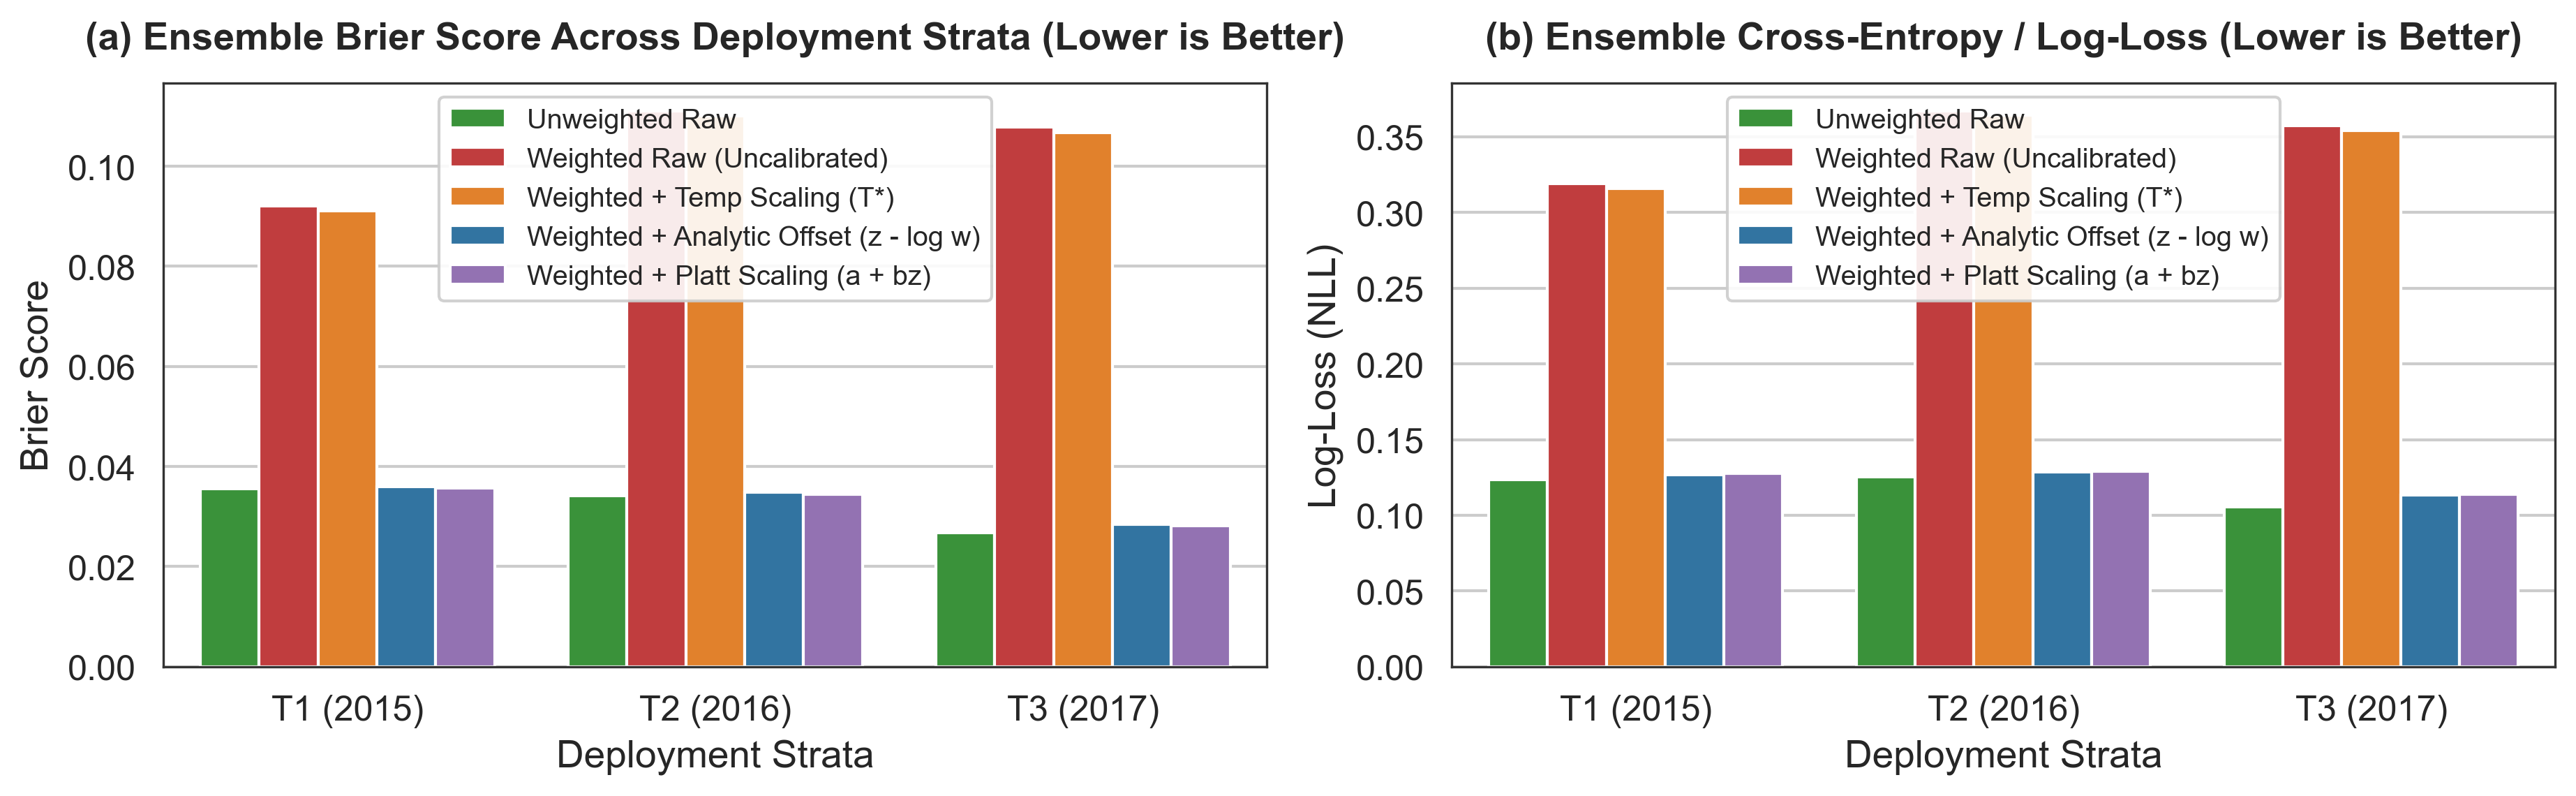
\includegraphics[width=0.85\textwidth]{figures/fig3_recalibration_comparison.png}
\caption{Multi-calibrator evaluation on Pleural Effusion for the DenseNet-121 3-seed ensemble across sequential deidentified-date strata ($T_1, T_2, T_3$), directly visualizing Table~\ref{tab:calibrator_comparison}. (a) Brier score and (b) Log-loss. Temperature scaling fails to reduce probability error in weighted models, whereas Analytic Offset ($z - \log w$) and Platt Scaling eliminate 74\% of Brier error, matching unweighted models.}
\label{fig:calibrator_comparison}
\end{figure*}

\section{Experimental Results}

\subsection{Experimental Matrix: Discrimination vs. Calibration Trajectories}
Table~\ref{tab:factorial_matrix} presents the comprehensive evaluation of the $2 \times 2$ experimental design comprising two architectures and two loss objectives (with three independently trained random seed replications per configuration, 12 models total) for Pleural Effusion, Cardiomegaly, and Pneumonia across chronological strata $T_1, T_2, T_3$.

\subsubsection{Discrimination Attenuation}
Both architectures exhibit moderate attenuation in AUROC across subsequent deidentified-date cohort strata. For DenseNet-121 on Pleural Effusion, AUROC decreases from $0.9335 \pm 0.0052$ at $T_1$ to $0.8731 \pm 0.0120$ at $T_3$ ($\Delta\text{AUROC} = -0.0604$). ResNet-50 exhibits an identical downward trajectory ($0.9295 \pm 0.0113 \to 0.8608 \pm 0.0190$, $\Delta\text{AUROC} = -0.0687$). This confirms that moderate discriminatory attenuation occurs across subsequent cohort strata, regardless of the training loss objective.

\subsubsection{Temporal Evolution of the Excess Calibration Penalty}
In stark contrast to discrimination, probability calibration diverges completely depending on the training loss function:
\begin{itemize}
    \item \textbf{Unweighted Models:} Brier scores are exceptionally low and actually \textit{improve} across subsequent strata for conditions with falling prevalence. For unweighted DenseNet-121 on Pleural Effusion, the Brier score improves from $0.0369 \pm 0.0029$ ($T_1$) to $0.0279 \pm 0.0009$ ($T_3$), while Equal-Mass ECE decreases from $0.0232$ to $0.0090$.
    \item \textbf{Positive-Weighted Models:} Brier scores are dramatically elevated and appear to degrade across subsequent cohort strata ($0.1081 \pm 0.0394 \to 0.1254 \pm 0.0456$ for DenseNet-121; $0.1256 \pm 0.0325 \to 0.1392 \pm 0.0310$ for ResNet-50). ECE exceeds 22\% across all held-out deidentified-date strata.
\end{itemize}

To track how this calibration disparity evolves across sequential deidentified-date cohort strata, we evaluate the excess calibration penalty $\Delta\text{Brier} = \text{Brier}_{\text{weighted}} - \text{Brier}_{\text{unweighted}}$ across sequential strata:
\begin{itemize}
    \item \textbf{Pleural Effusion (Prevalence Declines: $5.27\% \to 4.44\% \to 3.49\%$):} The excess calibration penalty of positive weighting expands monotonically across cohorts, from $\Delta\text{Brier} = +0.0712 \pm 0.0413$ in $T_1$ to $+0.0932 \pm 0.0428$ in $T_2$ and $+0.0975 \pm 0.0454$ in $T_3$.
    \item \textbf{Cardiomegaly (Prevalence Increases: $7.82\% \to 10.58\% \to 10.59\%$):} The excess calibration penalty remains stable or slightly attenuates: $\Delta\text{Brier} = +0.0729 \pm 0.0255$ in $T_1$, $+0.0681 \pm 0.0329$ in $T_2$, and $+0.0683 \pm 0.0320$ in $T_3$.
    \item \textbf{Pneumonia (Prevalence Steady Low: $2.66\% \to 1.98\% \to 2.05\%$):} The penalty remains consistently elevated: $\Delta\text{Brier} = +0.1079 \pm 0.0526$ in $T_1$, $+0.1126 \pm 0.0552$ in $T_2$, and $+0.1112 \pm 0.0508$ in $T_3$.
\end{itemize}
This establishes the operational mechanism: a static training-induced positive logit offset produces surplus false-positive probability mass that is penalized more severely when deployment disease prevalence drops, expanding the apparent temporal calibration gap.

\begin{table*}[!t]
\caption{Experimental Matrix Evaluation: Primary Longitudinal Performance across Architectures, Loss Objectives, and Thoracic Pathologies (Strata $T_1 \to T_3$). Values represent mean $\pm$ standard deviation across three independently trained random seeds ($S \in \{42, 123, 2026\}$). Complete 17-column trajectories across all intermediate deployment strata ($T_1, T_2, T_3$) and log-loss metrics are detailed in Supplementary Table~S3.}
\label{tab:factorial_matrix}
\centering
\small
\resizebox{\textwidth}{!}{%
\begin{tabular}{lllccccc}
\toprule
\textbf{Architecture} & \textbf{Objective} & \textbf{Pathology} & \textbf{AUROC ($T_1 \to T_3$)} & \textbf{$\Delta\text{AUROC}$} & \textbf{Brier ($T_1 \to T_3$)} & \textbf{$\Delta\text{Brier}$} & \textbf{ECE $T_3$} \\
\midrule
DenseNet-121 & Unweighted BCE & Pleural Effusion & 0.934 $\to$ 0.873 & -0.060 & 0.037 $\to$ 0.028 & -0.009 & 0.0090 \\
DenseNet-121 & Unweighted BCE & Cardiomegaly & 0.908 $\to$ 0.902 & -0.006 & 0.053 $\to$ 0.068 & +0.015 & 0.0210 \\
DenseNet-121 & Unweighted BCE & Pneumonia & 0.847 $\to$ 0.865 & +0.017 & 0.024 $\to$ 0.019 & -0.005 & 0.0095 \\
DenseNet-121 & Unweighted BCE & Edema* & 0.540 $\to$ -- & -- & 0.002 $\to$ 0.000 & -0.002 & 0.0029 \\
\midrule
DenseNet-121 & Pos-Weighted BCE & Pleural Effusion & 0.906 $\to$ 0.839 & -0.067 & 0.108 $\to$ 0.125 & +0.017 & 0.2227 \\
DenseNet-121 & Pos-Weighted BCE & Cardiomegaly & 0.874 $\to$ 0.858 & -0.016 & 0.126 $\to$ 0.136 & +0.010 & 0.1969 \\
DenseNet-121 & Pos-Weighted BCE & Pneumonia & 0.818 $\to$ 0.842 & +0.024 & 0.131 $\to$ 0.130 & -0.002 & 0.2425 \\
DenseNet-121 & Pos-Weighted BCE & Edema* & 0.612 $\to$ -- & -- & 0.061 $\to$ 0.064 & +0.002 & 0.1274 \\
\midrule
ResNet-50 & Unweighted BCE & Pleural Effusion & 0.930 $\to$ 0.861 & -0.069 & 0.037 $\to$ 0.028 & -0.009 & 0.0132 \\
ResNet-50 & Unweighted BCE & Cardiomegaly & 0.890 $\to$ 0.879 & -0.011 & 0.057 $\to$ 0.071 & +0.014 & 0.0175 \\
ResNet-50 & Unweighted BCE & Pneumonia & 0.843 $\to$ 0.880 & +0.037 & 0.024 $\to$ 0.019 & -0.005 & 0.0106 \\
ResNet-50 & Unweighted BCE & Edema* & 0.556 $\to$ -- & -- & 0.002 $\to$ 0.000 & -0.002 & 0.0017 \\
\midrule
ResNet-50 & Pos-Weighted BCE & Pleural Effusion & 0.879 $\to$ 0.819 & -0.060 & 0.126 $\to$ 0.139 & +0.014 & 0.2751 \\
ResNet-50 & Pos-Weighted BCE & Cardiomegaly & 0.830 $\to$ 0.799 & -0.031 & 0.142 $\to$ 0.152 & +0.011 & 0.2338 \\
ResNet-50 & Pos-Weighted BCE & Pneumonia & 0.835 $\to$ 0.823 & -0.012 & 0.167 $\to$ 0.169 & +0.002 & 0.3253 \\
ResNet-50 & Pos-Weighted BCE & Edema* & 0.549 $\to$ -- & -- & 0.069 $\to$ 0.075 & +0.005 & 0.1670 \\
\bottomrule
\end{tabular}

}
\end{table*}

\subsection{Multi-Calibrator Comparison}
Table~\ref{tab:calibrator_comparison} and Fig.~\ref{fig:calibrator_comparison} present the multi-calibrator benchmark for Pleural Effusion on the 3-seed ensemble across 2,000 patient-clustered bootstrap resamples, including Cox calibration regression intercept ($\alpha$) and slope ($\beta$) parameters.

\begin{table*}[!t]
\caption{Multi-Calibrator Comparison on Pleural Effusion: Deidentified-Date Ensemble Performance, Calibration Intercept ($\alpha$), Slope ($\beta$), and Paired Bootstrap Contrasts. Complete 12-column factorial evaluation across all intermediate strata and log-loss is provided in Supplementary Table~S4.}
\label{tab:calibrator_comparison}
\centering
\small
\resizebox{\textwidth}{!}{%
\begin{tabular}{lllccccc}
\toprule
\textbf{Architecture} & \textbf{Loss Objective} & \textbf{Calibrator} & \textbf{Brier ($T_1 \to T_3$)} & \textbf{$T_3$ $\alpha$} & \textbf{$T_3$ $\beta$} & \textbf{$T_3$ ECE} & \textbf{$T_3\ \Delta\text{Brier}$ vs Raw [95\% CI]} \\
\midrule
DenseNet-121 & Weighted BCE & Raw (Uncalibrated) & 0.092 $\to$ 0.108 & -2.964 & 1.048 & 0.2227 & -- \\
DenseNet-121 & Weighted BCE & Temperature Scaling ($T^*$) & 0.091 $\to$ 0.107 & -2.962 & 1.029 & 0.2190 & -0.0011 [-0.0014, -0.0009] \\
DenseNet-121 & Weighted BCE & Analytic Offset ($z - \log w$) & 0.036 $\to$ 0.028 & -0.445 & 0.929 & 0.0126 & \textbf{-0.0795} [-0.0893, -0.0697] \\
DenseNet-121 & Weighted BCE & Platt Scaling ($a + bz$) & 0.036 $\to$ 0.028 & -0.229 & 1.128 & 0.0176 & \textbf{-0.0798} [-0.0894, -0.0702] \\
DenseNet-121 & Unweighted BCE & Raw Baseline & 0.036 $\to$ 0.027 & +0.147 & 1.044 & 0.0040 & -- \\
\midrule
ResNet-50 & Weighted BCE & Raw (Uncalibrated) & 0.110 $\to$ 0.123 & -2.853 & 1.950 & 0.2751 & -- \\
ResNet-50 & Weighted BCE & Temperature Scaling ($T^*$) & 0.088 $\to$ 0.101 & -2.608 & 1.184 & 0.1993 & -0.0220 [-0.0241, -0.0198] \\
ResNet-50 & Weighted BCE & Analytic Offset ($z - \log w$) & 0.040 $\to$ 0.029 & +1.075 & 1.405 & 0.0158 & \textbf{-0.0936} [-0.1022, -0.0844] \\
ResNet-50 & Weighted BCE & Platt Scaling ($a + bz$) & 0.038 $\to$ 0.030 & -0.191 & 1.178 & 0.0223 & \textbf{-0.0930} [-0.1007, -0.0849] \\
ResNet-50 & Unweighted BCE & Raw Baseline & 0.036 $\to$ 0.027 & -0.077 & 1.095 & 0.0109 & -- \\
\bottomrule
\end{tabular}

}
\end{table*}

\subsubsection{Temperature Scaling Analysis}
For weighted DenseNet-121, temperature scaling optimizes $T^* \approx 1.0$, producing an uncalibrated $T_3$ Brier score of $0.1067$ compared to raw $0.1079$. The paired bootstrap contrast on the ensemble is $\Delta\text{Brier} = -0.0011$ [95\% CI: $-0.0014, -0.0009$], with the calibration intercept remaining severely displaced ($\alpha = -2.9615$ vs. raw $-2.9638$). For ResNet-50, temperature scaling achieves a modest variance adjustment ($\Delta\text{Brier} = -0.0220$ [95\% CI: $-0.0241, -0.0198$]), but leaves the underlying intercept discrepancy uncorrected ($\alpha = -2.6080$ vs. raw $-2.8526$). This demonstrates that temperature scaling provides limited or architecture-dependent empirical scaling, but cannot resolve the structural intercept displacement induced by positive loss weighting.

\subsubsection{Offset Correction and Parity Restoration}
The training positive weight for Pleural Effusion is $w = 21.51$, yielding an analytic logit offset of $\log w = +3.068$. Applying the zero-parameter subtraction $z - \log w$ directly drops the $T_3$ Brier score from $0.1079$ to $0.0284$ ($\Delta\text{Brier} = -0.0795$ [95\% CI: $-0.0893, -0.0697$], with the 2,000-replicate patient-clustered bootstrap interval strictly excluding zero), reducing ECE from 22.3\% to 1.26\%. Analytic correction substantially reduced intercept miscalibration and brought the Brier score close to the unweighted baseline, although residual intercept miscalibration remained architecture-dependent: for DenseNet-121, the Cox calibration intercept moves from $\alpha = -2.9638$ directly to $\alpha = -0.4451$ while perfectly preserving the calibration slope ($\beta = 0.9292$), whereas for ResNet-50 the corrected intercept is $\alpha = +1.0751$.

Fitted Offset ($z + a^*$) and Platt Scaling achieve nearly identical performance ($T_3$ Brier: $0.0289$ and $0.0281$; $\Delta\text{Brier} = -0.0790$ [95\% CI: $-0.0885, -0.0696$] and $-0.0798$ [95\% CI: $-0.0894, -0.0702$]). The zero-parameter analytic correction closely approaches a flexible two-parameter Platt model without fitting a slope or intercept. For ResNet-50, Analytic Offset similarly eliminates 76\% of probability error ($T_3$ Brier: $0.1227 \to 0.0291$, $\Delta\text{Brier} = -0.0936$ [95\% CI: $-0.1022, -0.0844$]), confirming that intercept neutralization is architecturally universal.

\subsubsection{\texorpdfstring{Empirical Verification of Logit Offset: $z_w - z_u \approx \log w$}{Empirical Verification of Logit Offset: z_w - z_u approx log w}}
\label{sec:logit_offset}
To directly validate the theoretical prediction of Equation~(\ref{eq:bayes_logit}) in finite deep neural networks, Fig.~\ref{fig:logit_offset} plots the empirical distributions of logit differences $\Delta z(x) = \bar{z}_w(x) - \bar{z}_u(x)$ evaluated across all 16,604 image-architecture ensemble pairs (averaged across the three seed-matched model pairs) against the theoretical reference value $\log w$:
\begin{itemize}
    \item \textbf{Pleural Effusion ($\log w = 3.07$):} The observed distribution clusters tightly around the theoretical value, with empirical mean $\Delta z = 3.29 \pm 0.81$ and median $3.25$ (interquartile range [IQR]: $2.77$--$3.79$), exhibiting an average bias of only $+0.22$ logit units.
    \item \textbf{Pneumonia ($\log w = 3.99$):} Observed mean $\Delta z = 3.83 \pm 0.74$ and median $3.84$ (IQR: $3.34$--$4.32$), closely matching theory with a minimal discrepancy of $-0.16$ logit units.
    \item \textbf{Cardiomegaly ($\log w = 2.25$):} Observed mean $\Delta z = 2.64 \pm 1.04$ and median $2.60$ (IQR: $1.91$--$3.31$), bias $+0.39$ logit units.
    \item \textbf{Edema (Extreme Imbalance: $w = 1091.3, \log w = 7.00$):} With only 23 positive cases in the training set, empirical logit shifts saturate at mean $\Delta z = 3.69 \pm 1.47$ (median $3.46$, IQR: $2.63$--$4.58$). Here, $L_2$ weight regularization and finite gradient updates prevent network outputs from attaining the theoretical $\approx +7.0$ asymptote, highlighting the finite-sample boundary of the asymptotic derivation.
\end{itemize}

\begin{figure*}[!t]
\centering
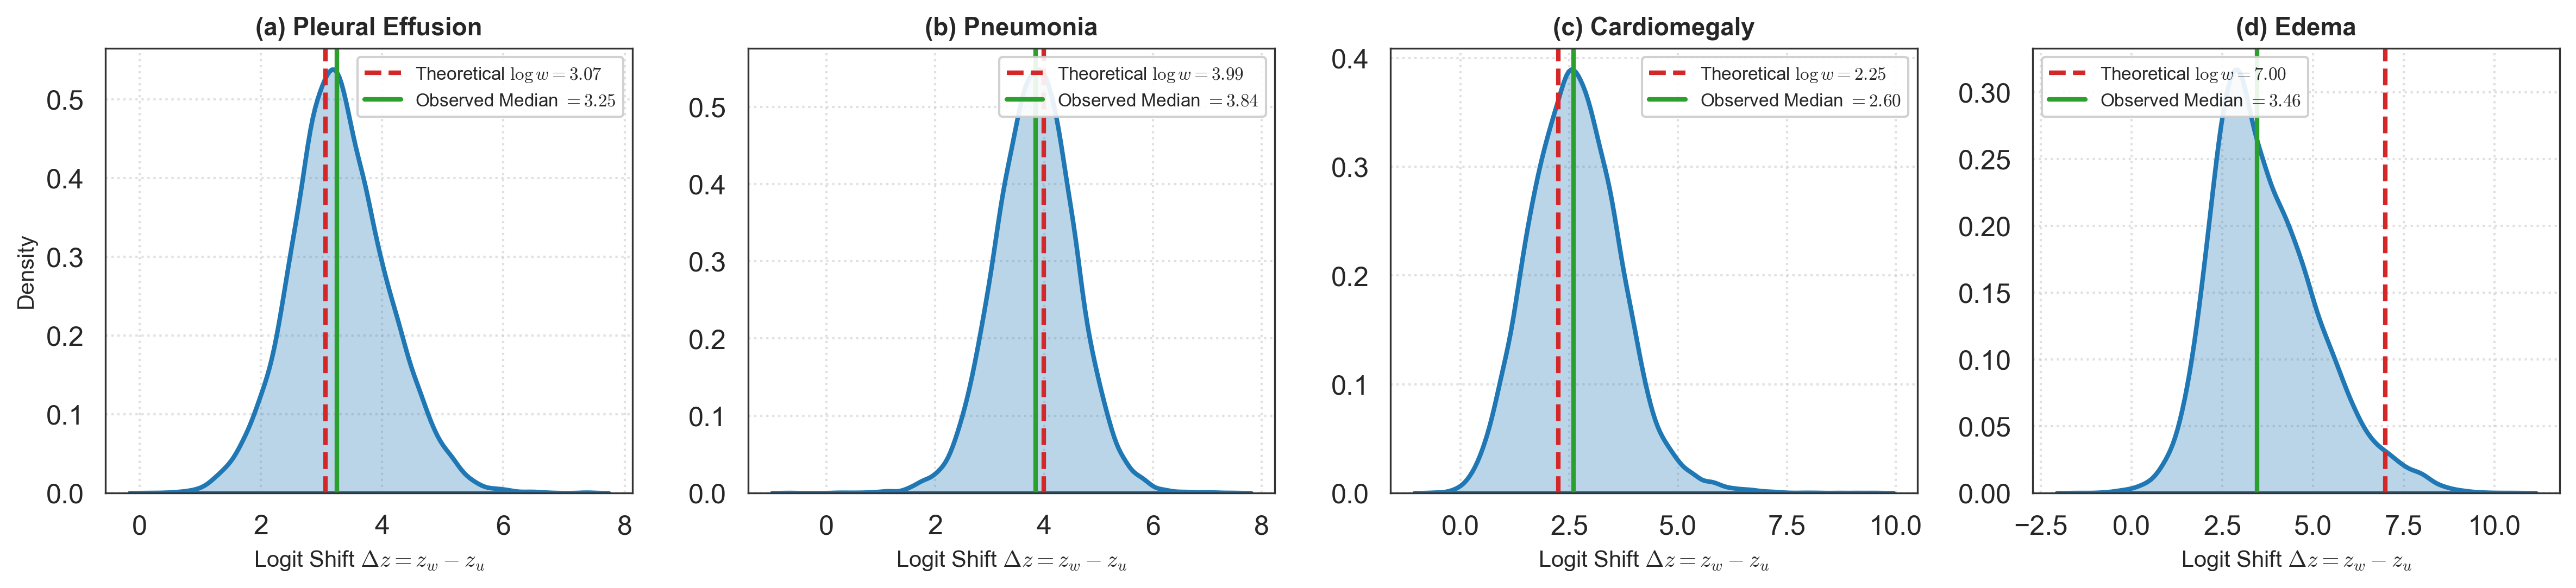
\includegraphics[width=\textwidth]{figures/fig6_logit_offset_verification.png}
\caption{Empirical verification of theoretical logit shift ($z_w - z_u \approx \log w$) across 16,604 held-out deidentified-date image evaluations ($8,302\text{ images} \times 2\text{ architectures}$, with $\Delta z$ computed as the mean difference across the three seed-matched weighted/unweighted model pairs). Kernel density estimates (blue) of observed logit differences between positive-weighted and unweighted models cluster tightly around the theoretical population attractor $\log w$ (dashed red line; observed median in solid green) across Pleural Effusion (a), Pneumonia (b), and Cardiomegaly (c). For Edema (d), extreme training class scarcity ($w > 1000$) induces optimization saturation, bounding empirical shifts near $+3.69$.}
\label{fig:logit_offset}
\end{figure*}

\subsubsection{Reliability Diagrams}
Figure~\ref{fig:reliability} shows reliability diagrams across sequential deidentified-date strata $T_1, T_2, T_3$ using adaptive 10-bin equal-mass partitioning. Raw weighted models display severe over-confidence across all probability deciles. Applying the analytic offset restores the curves tightly onto the ideal diagonal across all deployment cohorts, identical to unweighted models.

\begin{figure}[!b]
\centering
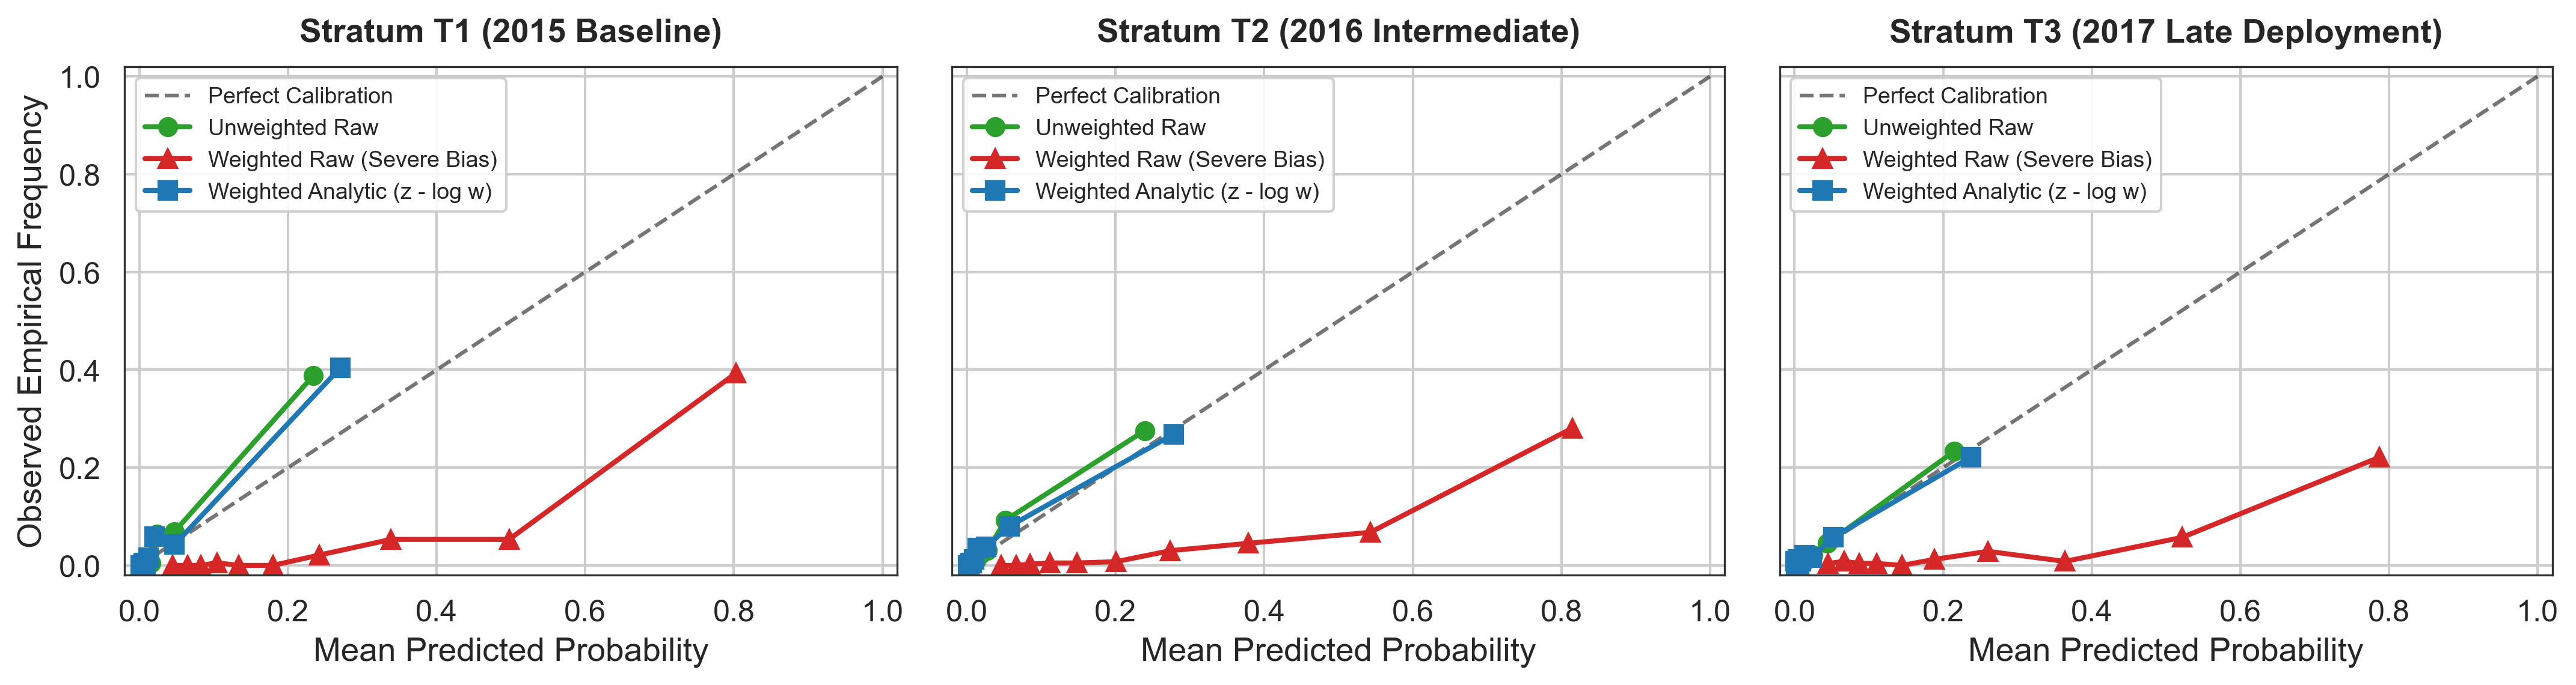
\includegraphics[width=0.75\linewidth]{figures/fig5_reliability_diagrams.png}
\caption{Reliability diagrams for Pleural Effusion (DenseNet-121 3-seed ensemble) across held-out deidentified-date strata ($T_1, T_2, T_3$). Raw weighted models (red) severely over-predict event probabilities across all bins. Analytic offset calibration (blue) and unweighted models (green) remain tightly calibrated to the ideal diagonal across all deployment windows.}
\label{fig:reliability}
\end{figure}

\subsection{Selective Prediction and Workload Triage Simulation}
Table~\ref{tab:selective_prediction} and Fig.~\ref{fig:selective_prediction} summarize the selective triage simulation on the later held-out deidentified-date stratum $T_3$ ($N = 2,436$ radiographs, containing 85 true positive Pleural Effusion cases), explicitly accounting for retained positives, automated true positives, missed cases, and both retained and full-cohort triage sensitivities.

\begin{table*}[!t]
\caption{Selective Prediction and Reader Referral Triage Simulation on Later Held-Out Stratum $T_3$ ($N = 2,436$ Radiographs, 85 Positive Pleural Effusion Cases). Evaluated under matched Youden decision thresholds determined on development stratum $T_1$ across primary clinical operating regimes (100\%, 90\%, 80\%, 70\% coverage). Complete 24-row simulation across all coverage levels is detailed in Supplementary Table~S5.}
\label{tab:selective_prediction}
\centering
\small
\resizebox{\textwidth}{!}{%
\begin{tabular}{lllccccc}
\toprule
\textbf{Coverage} & \textbf{Referred (Workload)} & \textbf{Strategy} & \textbf{Automated FN (Missed)} & \textbf{Retained Sens.} & \textbf{Full Sens.} & \textbf{Retained AUROC} & \textbf{Retained Brier} \\
\midrule
100\% & 0 (0\%) & Weighted BCE (Raw) & 16.0 & 81.18\% & 81.18\% & 0.8691 & 0.1079 \\
100\% & 0 (0\%) & Weighted BCE (Analytic Corrected) & 16.0 & 81.18\% & 81.18\% & 0.8623 & 0.0284 \\
100\% & 0 (0\%) & Unweighted BCE (Raw) & 12.0 & 85.88\% & 85.88\% & 0.8806 & 0.0268 \\
\midrule
90\% & 243 (10\%) & Weighted BCE (Raw) & 14.0 & 82.93\% & 83.53\% & 0.8789 & 0.1062 \\
90\% & 243 (10\%) & Weighted BCE (Analytic Corrected) & 15.0 & 81.01\% & 82.35\% & 0.8735 & 0.0289 \\
90\% & 243 (10\%) & Unweighted BCE (Raw) & 12.0 & 84.62\% & 85.88\% & 0.8923 & 0.0266 \\
\midrule
80\% & 487 (20\%) & Weighted BCE (Raw) & 10.0 & 87.01\% & 88.24\% & 0.8882 & 0.1012 \\
80\% & 487 (20\%) & Weighted BCE (Analytic Corrected) & 15.0 & 77.61\% & 82.35\% & 0.8896 & 0.0264 \\
80\% & 487 (20\%) & Unweighted BCE (Raw) & 12.0 & 82.61\% & 85.88\% & 0.9027 & 0.0256 \\
\midrule
70\% & 730 (30\%) & Weighted BCE (Raw) & 7.0 & 89.39\% & 91.76\% & 0.8997 & 0.0956 \\
70\% & 730 (30\%) & Weighted BCE (Analytic Corrected) & 13.0 & 70.45\% & 84.71\% & 0.8876 & 0.0178 \\
70\% & 730 (30\%) & Unweighted BCE (Raw) & 11.0 & 78.00\% & 87.06\% & 0.9051 & 0.0194 \\
70\% & 730 (30\%) & Random Deferral Baseline & 11.3 & 80.99\% & 86.69\% & -- & 0.1081 \\
\bottomrule
\end{tabular}

}
\end{table*}

\begin{figure*}[!t]
\centering
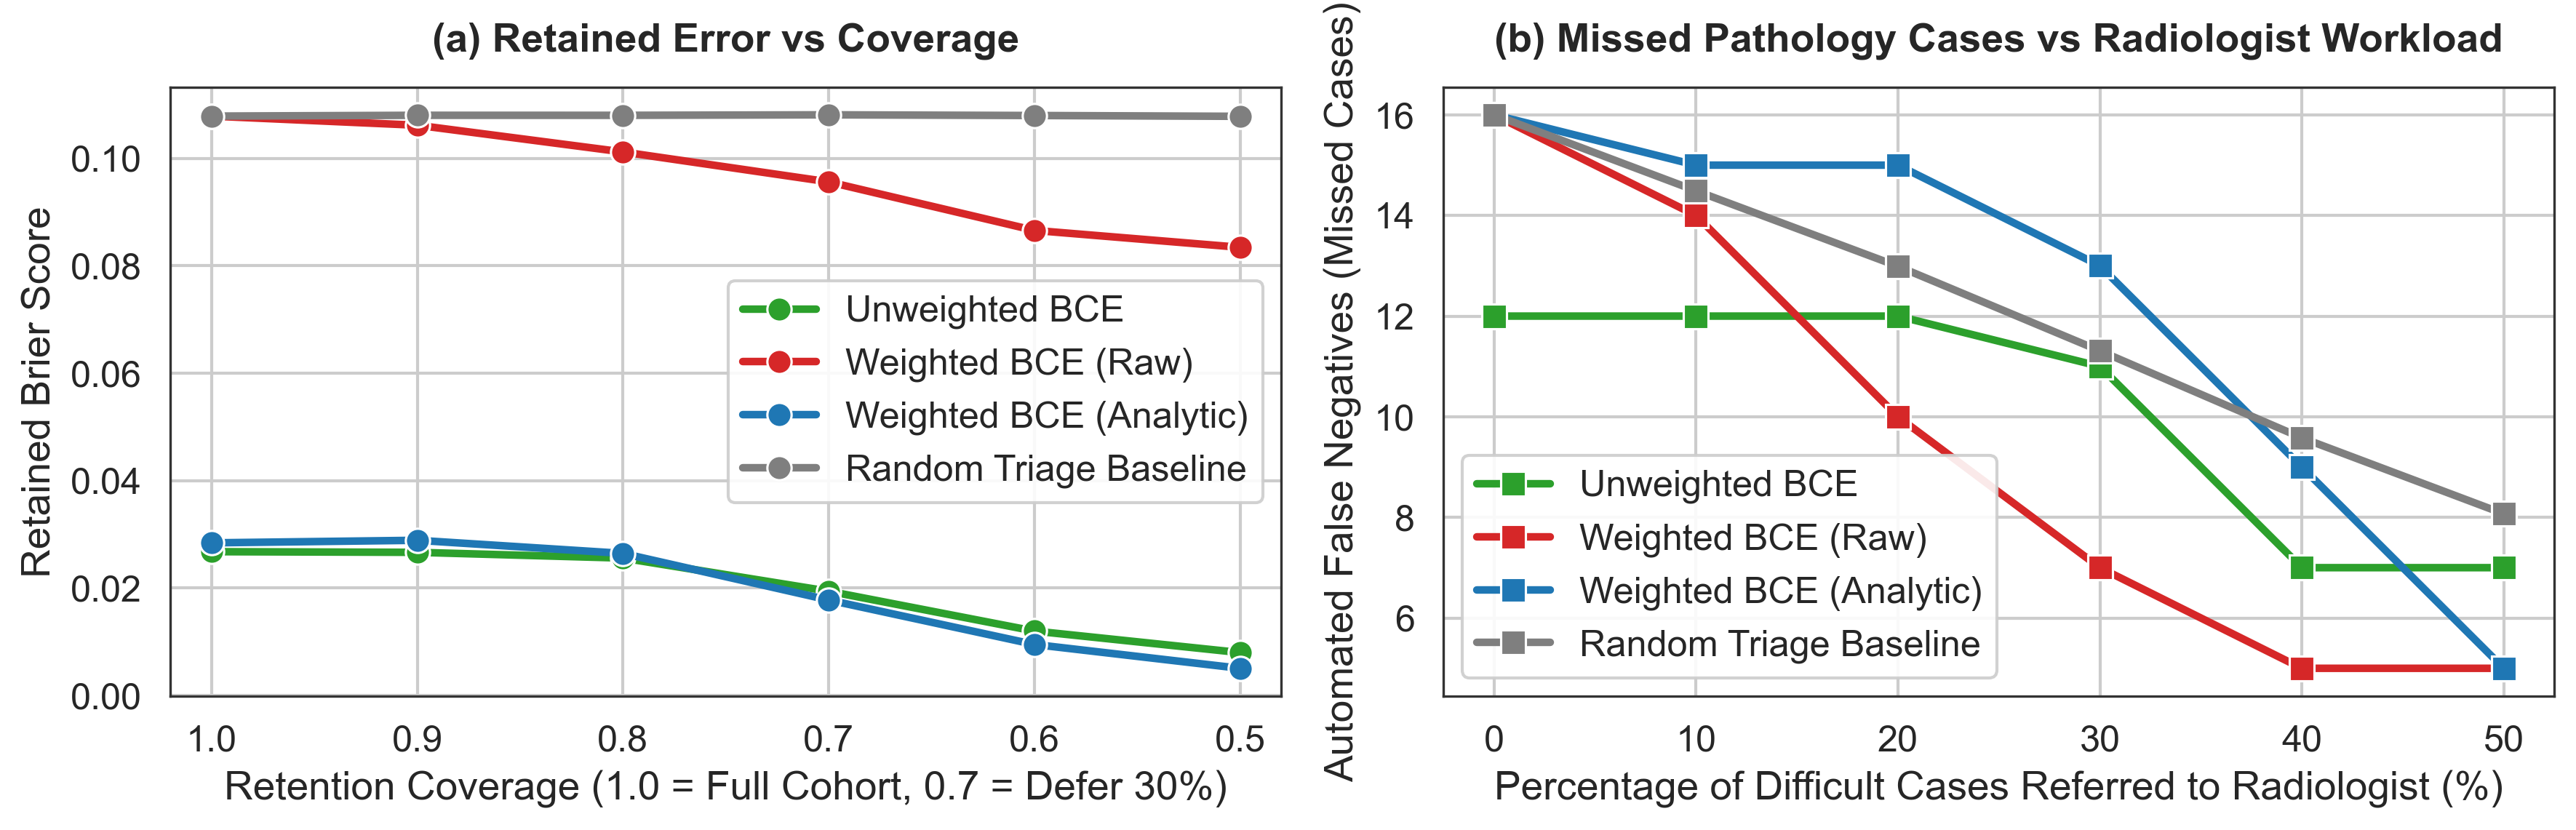
\includegraphics[width=0.85\textwidth]{figures/fig4_selective_risk_coverage.png}
\caption{Selective prediction evaluation on later held-out stratum $T_3$ with matched development thresholds (Table~\ref{tab:selective_prediction}). Left: Risk-coverage curves demonstrating that selective deferral steadily reduces Brier error across all models as ambiguous cases are referred. Right: Reader referral workload vs. automated false negatives, illustrating the distinct operational behaviors of raw weighted models (halving missed cases to 7.0 under 30\% referral) and analytic corrected models (optimizing probability accuracy with Brier 0.0178).}
\label{fig:selective_prediction}
\end{figure*}

At 100\% coverage (full automation), the raw weighted model incurs 16.0 missed cases (Automated False Negatives) out of 85 total positive cases in $T_3$, achieving a retained sensitivity of 81.18\%, AUROC of 0.8691, and Brier score of 0.1079. Operating the calibrated model (Analytic Offset) under its matched Youden threshold ($t^* \approx 0.022$) yields identical sensitivity (81.18\%) and 16.0 missed cases, but with an almost four-fold lower Brier score of 0.0284. The unweighted raw model achieves 12.0 missed cases (sensitivity 85.88\%, AUROC 0.8806, Brier 0.0268).

Under selective triage based on prediction margin from each method's operational decision cutoff:
\begin{itemize}
    \item \textbf{Raw Weighted BCE (Triage-Optimized):} At 90\% coverage (243 borderline radiographs referred to a reader), automated false negatives decrease to 14.0 (full-cohort system sensitivity 83.53\%). At 80\% coverage (487 referred), false negatives drop to 10.0 (system sensitivity 88.24\%). At 70\% coverage (730 examinations referred, 30\% workload), 66 true positive cases remain in the automated fraction and 59 are correctly flagged as positive, cutting missed cases by more than half to 7.0 (retained sensitivity 89.39\%, full-cohort triage sensitivity 91.76\%), outperforming random triage (11.3 missed cases). However, retained probabilities remain uncalibrated and biased high (Brier score 0.0956).
    \item \textbf{Analytic Corrected BCE (Probability-Optimized):} Operating under its matched threshold ($t^* \approx 0.022$), the calibrated model achieves an exceptional Brier score of 0.0178 at 70\% coverage (a $>5$-fold reduction in probability error relative to the raw model). However, because predicted probabilities are concentrated near true clinical prevalence ($p \in [0.001, 0.05]$), the distance normalization in Equation~(\ref{eq:uncertainty}) assigns low uncertainty to low-probability false negatives ($\hat{p} \ll t^*$). Consequently, subtle false negatives are retained rather than referred, leaving 13.0 automated false negatives among 44 retained positives (retained sensitivity 70.45\%, full-cohort triage sensitivity 84.71\%) at 70\% coverage.
    \item \textbf{Raw Unweighted BCE:} At 70\% coverage, the unweighted model retains 50 positive cases, correctly flags 39, and incurs 11.0 automated false negatives with retained Brier score 0.0194 (retained sensitivity 78.00\%, full-cohort triage sensitivity 87.06\%).
\end{itemize}

Importantly, these empirical results expose an operational trade-off in machine learning deployment: post-hoc probability calibration (Analytic Offset) is essential for accurate risk estimation and prognosis, dropping Brier scores to near-optimal levels ($0.0284 \to 0.0178$); conversely, threshold-margin selective triage on raw positive-weighted models is effective for recall-oriented screening referral (cutting missed cases from 16 to 7), but yields biased probabilities. Because the analytic logit transformation $z \mapsto z - \log w$ is strictly monotonic, any ranking-based decision rule under an equivalent quantile threshold produces identical patient prioritization. The operational divergence observed in Table~\ref{tab:selective_prediction} arises specifically because the uncertainty triage metric $u(x)$ in Equation~(\ref{eq:uncertainty}) measures distance relative to the operational decision cutoff $t^*$ determined on development stratum $T_1$. For calibrated models, $t^* \approx 0.022$ aligns with low clinical prevalence, causing low-probability false negatives ($\hat{p} \ll t^*$) to exhibit low relative uncertainty and remain in the automated pool; for raw weighted models, the elevated threshold ($t^* \approx 0.33$) places borderline cases within the referral margin. Consequently, selective referral performance is fundamentally policy-dependent: calibrated probabilities are required for valid decision-theoretic risk stratification, whereas raw weighted models with threshold-margin triage act as a heuristic for recall-oriented screening. Crucially, neither system achieves zero false negatives, refuting unsubstantiated claims of complete error elimination in autonomous settings.

\subsection{Cross-Institutional External Evaluation (MIMIC-CXR-JPG)}
The external MIMIC-CXR-JPG cohort comprised 3,403 frontal radiographs from 3,041 studies and 289 patients, with complete image availability. Rather than asserting turnkey diagnostic transportability—as confirmed by moderate discrimination for Pleural Effusion (AUROC $0.688$ [95\% CI: $0.656, 0.717$] for unweighted DenseNet-121 and $0.677$ [95\% CI: $0.645, 0.709$] for unweighted ResNet-50), weak discrimination for Pneumonia ($0.583$--$0.607$) and Edema ($0.516$--$0.581$), and near-chance discrimination for Cardiomegaly ($0.519$--$0.525$, with patient-clustered 95\% CIs spanning $0.50$)—this experiment functions as a rigorous external stress-test of whether loss-induced logit distortion and zero-parameter offset recovery persist across distinct health systems, acquisition hardware, and report extraction pipelines. Negative Brier skill scores ($\text{BSS} < 0$) across all configurations indicated that transported BRAX probabilities were less accurate than a local MIMIC prevalence-only reference model ($\text{Brier}_{\text{null}} = \pi(1 - \pi)$), demonstrating substantial cross-institutional baseline calibration shift.

Evaluating paired analytic offset recalibration ($\bar{p}_{\text{corrected}} = \frac{1}{3}\sum \sigma(z_s - \log w)$) on positive-weighted models demonstrated statistically significant reductions in Brier error for Cardiomegaly ($\Delta\text{Brier} = -0.0579$ [95\% CI: $-0.0790, -0.0349$] on DenseNet-121; $-0.0611$ [95\% CI: $-0.0818, -0.0415$] on ResNet-50) and Pneumonia ($\Delta\text{Brier} = -0.0095$ [95\% CI: $-0.0170, -0.0016$] on DenseNet-121; $-0.0155$ [95\% CI: $-0.0254, -0.0059$] on ResNet-50), with consistent point-estimate error reduction on Pleural Effusion ($-0.0084$ and $-0.0109$). On MIMIC-CXR-JPG, subtraction of the full theoretical offset worsened the Edema Brier score. This result is consistent with over-correction when the empirically realized finite-network shift is smaller than the theoretical $\log w$; however, cross-institutional covariate and label differences prevent attribution of this external result uniquely to optimization saturation. Because logit subtraction $z - \log w$ is strictly monotonic, discriminatory ranking (AUROC) was perfectly preserved across all pathologies.

To evaluate sensitivity to repeated within-patient examinations and multi-image studies, we conducted a parallel sensitivity analysis aggregated strictly at the diagnostic study level ($N = 3,041$ studies across $N = 289$ patients) using maximum probability pooling ($\max_i p_i$). Study-level discrimination was concordant with image-level evaluation across all pathologies: Pleural Effusion AUROC was $0.695$ [95\% CI: $0.663, 0.723$] for unweighted DenseNet-121 and $0.682$ [95\% CI: $0.650, 0.714$] for ResNet-50; Cardiomegaly AUROC was $0.526$ [95\% CI: $0.497, 0.559$] and $0.521$ [95\% CI: $0.494, 0.548$]; Pneumonia AUROC was $0.608$ [95\% CI: $0.562, 0.650$] and $0.584$ [95\% CI: $0.543, 0.624$]; and Edema AUROC was $0.565$ [95\% CI: $0.528, 0.600$] and $0.516$ [95\% CI: $0.480, 0.553$], with study-level null Brier baselines of $0.2196$ (Effusion), $0.1951$ (Cardiomegaly), $0.0913$ (Pneumonia), and $0.1697$ (Edema). Furthermore, paired analytic recalibration on positive-weighted models demonstrated identical calibration invariance at study level: statistically significant Brier reductions were reproduced for Cardiomegaly ($\Delta\text{Brier} = -0.0601$ [95\% CI: $-0.0814, -0.0367$] on DenseNet-121; $-0.0642$ [95\% CI: $-0.0852, -0.0434$] on ResNet-50) and Pneumonia ($\Delta\text{Brier} = -0.0100$ [$-0.0179, -0.0018$]; $-0.0163$ [$-0.0267, -0.0068$]), with consistent point-estimate reductions for Pleural Effusion ($-0.0102$ and $-0.0118$; Supplementary Table~S2). This qualitative concordance confirms that cross-institutional discrimination patterns and recalibration effects are preserved when aggregating by diagnostic study.

\begin{table*}[!t]
\caption{Cross-Institutional External Validation on the Official MIMIC-CXR-JPG Frontal Test Cohort ($N = 3,403$ Images from $3,041$ Studies Across $N = 289$ Unique Patients). Primary experimental evaluation of paired zero-parameter analytic logit recalibration ($\bar{p}_{\text{raw}} = \frac{1}{3}\sum \sigma(z_s) \to \bar{p}_{\text{corr}} = \frac{1}{3}\sum \sigma(z_s - \log w)$) on 3-seed ensembles trained with positive-weighted BCE. Evaluated with empirical prevalence ($\pi$), local null reference baseline ($\text{Brier}_{\text{null}} = \pi(1-\pi)$), patient-clustered 1,000-replicate bootstrap 95\% confidence intervals, Brier skill score ($\text{BSS} = 1 - \text{Brier}/\text{Brier}_{\text{null}}$), and paired contrast ($\Delta\text{Brier} = \text{Brier}_{\text{corr}} - \text{Brier}_{\text{raw}}$). The complete 16-row factorial comparison with unweighted BCE baselines is detailed in Supplementary Table~S1, and study-level sensitivity analysis is detailed in Supplementary Table~S2.}
\label{tab:mimic_external_validation}
\centering
\small
\resizebox{\textwidth}{!}{%
\begin{tabular}{llccccccc}
\toprule
\textbf{Architecture} & \textbf{Pathology} & \textbf{Prevalence ($\pi$)} & \textbf{$\text{Brier}_{\text{null}}$} & \textbf{AUROC [95\% CI]} & \textbf{Brier (Raw $\to$ Corr)} & \textbf{$\Delta\text{Brier}$ [95\% CI]} & \textbf{$\text{BSS}$ (Raw $\to$ Corr)} \\
\midrule
DenseNet-121 & Pleural Effusion & 32.18\% & 0.2182 & 0.668 [0.636, 0.700] & 0.2536 $\to$ 0.2451 & -0.0084 [-0.0401, +0.0240] & -0.162 $\to$ -0.123 \\
DenseNet-121 & Cardiomegaly & 26.33\% & 0.1940 & 0.525 [0.492, 0.558] & 0.2907 $\to$ 0.2328 & \textbf{-0.0579} [-0.0790, -0.0349] & -0.499 $\to$ -0.200 \\
DenseNet-121 & Pneumonia & 10.05\% & 0.0904 & 0.598 [0.553, 0.639] & 0.1078 $\to$ 0.0983 & \textbf{-0.0095} [-0.0170, -0.0016] & -0.192 $\to$ -0.087 \\
DenseNet-121 & Edema & 21.33\% & 0.1678 & 0.581 [0.549, 0.611] & 0.1914 $\to$ 0.2131 & +0.0217 [+0.0118, +0.0307] & -0.141 $\to$ -0.270 \\
\midrule
ResNet-50 & Pleural Effusion & 32.18\% & 0.2182 & 0.620 [0.588, 0.653] & 0.2665 $\to$ 0.2557 & -0.0109 [-0.0417, +0.0253] & -0.221 $\to$ -0.172 \\
ResNet-50 & Cardiomegaly & 26.33\% & 0.1940 & 0.522 [0.491, 0.552] & 0.2822 $\to$ 0.2211 & \textbf{-0.0611} [-0.0818, -0.0415] & -0.455 $\to$ -0.140 \\
ResNet-50 & Pneumonia & 10.05\% & 0.0904 & 0.589 [0.545, 0.629] & 0.1137 $\to$ 0.0982 & \textbf{-0.0155} [-0.0254, -0.0059] & -0.257 $\to$ -0.086 \\
ResNet-50 & Edema & 21.33\% & 0.1678 & 0.570 [0.538, 0.602] & 0.1929 $\to$ 0.2130 & +0.0201 [+0.0092, +0.0313] & -0.149 $\to$ -0.269 \\
\bottomrule
\end{tabular}%
}
\end{table*}

\section{Discussion}

\subsection{Disentangling Loss-Induced Probability Distortion from Deidentified-Date Cohort Shift}
A substantial body of recent literature in biomedical informatics has sounded alarms regarding temporal calibration decay in healthcare AI~\cite{guo2022evaluation, hinson2022multisite}. Our findings elucidate the mathematical and empirical mechanisms underlying these observations. It is critical to distinguish between discrimination loss and calibration error: our experiments confirm that moderate discrimination attenuation does occur across later deidentified-date cohort strata (AUROC decreases by approximately $0.06$ from $T_1$ to $T_3$ identically across both unweighted and weighted models in Table~\ref{tab:factorial_matrix}). However, the simultaneous perception of severe, progressive calibration collapse is largely an artifact of positive loss weighting compounded by shifting disease prevalence.

When practitioners train deep neural networks on highly imbalanced clinical datasets, positive loss weighting is frequently introduced to elevate minority-class sensitivity~\cite{rajpurkar2017chexnet}. However, as derived in Equation~(\ref{eq:bayes_logit}) and verified empirically in Fig.~\ref{fig:logit_offset}, this introduces a static logit shift $\approx \log w$. When evaluated on later cohort strata where disease prevalence shifts (e.g., Pleural Effusion prevalence declining from 5.27\% in $T_1$ to 3.49\% in $T_3$), this fixed positive offset generates surplus false-positive probability mass that compounds the apparent Brier error. Because standard post-hoc evaluation pipelines rely almost exclusively on temperature scaling---which cannot alter the logit intercept---evaluators observing deteriorating Brier scores have routinely attributed the failure to intrinsic model decay.

Our experiments provide direct evidence against this attribution. When the mathematical offset is neutralized ($z - \log w$), the apparent calibration decay vanishes: Brier scores decrease across subsequent strata, moving in lockstep with the unweighted baseline as disease prevalence drops. Thus, while discrimination attenuation reflects underlying dataset shift across cohort strata, severe calibration degradation is predominantly an uncorrected post-training calibration bias that can be decoupled and resolved analytically.

\subsection{Relationship to Prior Work on Class Weights and Likelihood Recovery}
Our theoretical analysis connects directly with the foundational work of Caplin, Martin, and Marx~\cite{caplin2022calibrating}, who demonstrated that training with class weights inherently corrupts probability calibration and established an inverse modeling method to recover undistorted likelihoods, illustrating their recovery technique on a static CheXNet pneumonia model. While Caplin et al. established that class weighting and raw calibration are fundamentally at odds in stationary settings, our study addresses critical dimensions left unexplored in prior theoretical treatments:
\begin{enumerate}
    \item \textbf{Resolution of the ``Temporal Calibration Decay'' Paradox:} Caplin et al. investigated stationary, single-split validation. We address the active clinical informatics debate regarding longitudinal stability~\cite{guo2022evaluation, hinson2022multisite, davis2020detection}, proving that apparent temporal calibration decay over chronological cohort strata ($T_1 \to T_3$) is driven by uncorrected training-loss offsets interacting with dynamic clinical prevalence rather than intrinsic temporal drift.
    \item \textbf{Structural Failure of Temperature Scaling:} While Caplin et al. focused on recovering likelihoods from weighted models, standard clinical vision pipelines continue to rely on temperature scaling~\cite{guo2017calibration}. We provide analytical and empirical proof that temperature scaling is structurally incapable of rectifying weighted models because it operates solely on logit dispersion while leaving the large negative calibration intercept ($\alpha \approx -2.96$) completely uncorrected.
    \item \textbf{Finite Neural Network Dynamics and Scarcity Bounds:} Unlike idealized asymptotic formulations, our 16,604 paired evaluations across DenseNet-121 and ResNet-50 (spanning 49,812 seed-level model runs) uncover where finite deep networks diverge from theory: while empirical shifts match $\log w$ across moderate-prevalence conditions, extreme class scarcity ($w > 1000$ in Edema) induces optimization saturation ($\Delta z \approx +3.69$ vs. theoretical $+7.00$) due to $L_2$ regularization and gradient clipping.
    \item \textbf{Cross-Institutional Stress-Testing:} Rather than asserting turnkey clinical transportability (given modest to near-chance external discrimination), we evaluate whether zero-parameter analytic logit correction ($z - \log w$) survives extreme multi-center stress-testing from BRAX ($N=40,523$, Brazil) to MIMIC-CXR ($N=3,403$, USA), delineating where loss correction successfully mitigates calibration error versus where cross-institutional domain shifts dominate.
    \item \textbf{Clinical Decision Triage vs. Probability Calibration:} Extending recent multi-dataset selective CXR investigations~\cite{aperstein2026knowing}, we operationalize the practical dilemma facing clinicians: while analytic correction ($z - \log w$) is strictly required for epidemiological risk stratification and prognosis (restoring Brier parity, consistent with plug-in probability recovery principles~\cite{piccininni2024understanding}), raw weighted models provide superior threshold-margin selective triage by halving automated false negatives under operational referral constraints.
\end{enumerate}

\subsection{Architectural Generalizability}
The observed phenomena are remarkably consistent across distinct deep learning architectures. Both DenseNet-121 (dense convolutional concatenation) and ResNet-50 (residual identity mapping) exhibit near-identical behavior:
\begin{itemize}
    \item Discrimination attenuation across later held-out strata is virtually indistinguishable between architectures ($\Delta\text{AUROC} = -0.0604$ vs. $-0.0687$).
    \item Both architectures experience severe raw calibration error under weighted BCE (raw ensemble Brier $0.1079$ vs $0.1227$ on $T_3$; $0.1254 \pm 0.0456$ vs $0.1392 \pm 0.0310$ across individual seeds), characterized by large negative calibration intercepts ($\alpha \approx -2.96$ and $-2.85$).
    \item For both architectures, Analytic Offset reduces total Brier score by approximately 74\% to 76\% ($\Delta\text{Brier} = -0.0795$ [95\% CI: $-0.0893, -0.0697$] for DenseNet-121 and $-0.0936$ [95\% CI: $-0.1022, -0.0844$] for ResNet-50), substantially reducing intercept miscalibration ($\alpha = -0.4451$ and $+1.0751$) while preserving calibration slopes ($\beta = 0.9292$ and $1.4052$). This confirms that logit-shift mechanics are universal across convolutional vision backbones, though residual intercept bias remains architecture-dependent.
\end{itemize}

\subsection{Simulated Human-in-the-Loop Triage and Operational Trade-offs}
In real-world clinical deployment workflows, autonomous decision-making must be evaluated through uncertainty-aware deferral simulations:
\begin{enumerate}
    \item \textbf{Risk Stratification and Prognosis:} Well-calibrated models are essential for automated rule-out and downstream risk scoring. Applying Analytic Offset ($z - \log w$) drops Brier error to 0.0178 at 70\% coverage, restoring reliable posterior probabilities aligned with true clinical prevalence.
    \item \textbf{High-Sensitivity Screening Referral:} In high-throughput screening where the primary objective is minimizing missed disease, threshold-margin selective triage on raw positive-weighted models cuts automated false negatives from 16 to 7 (full-cohort triage sensitivity 91.76\%) under a 30\% reader referral budget. However, because probabilities remain biased high (Brier 0.0956), these outputs should not be used as calibrated risks.
    \item \textbf{Zero-Parameter Operational Utility:} The analytic offset ($z - \log w$) requires zero retraining, zero validation optimization, and zero compute overhead, enabling immediate integration on edge inference devices.
\end{enumerate}

\subsection{Scope and Boundary of Findings and Limitations}
To establish the scope and boundary of findings, several important methodological and clinical limitations should be highlighted:
\begin{enumerate}
    \item \textbf{Report-Derived Label Noise:} Ground-truth labels in BRAX were generated via natural language processing from Portuguese text reports. Although validated against expert consensus, report-derived labels carry inherent extraction noise compared to dedicated multi-radiologist image re-reading.
    \item \textbf{Cross-Institutional Domain Gap and Modest Diagnostic Transportability:} Our external evaluation on MIMIC-CXR-JPG serves to stress-test calibration mechanics under severe domain shift rather than demonstrate ready-to-deploy clinical diagnostic transportability. Models achieved only modest discrimination for Pleural Effusion (AUROC $\approx 0.69$) and degraded near chance for Cardiomegaly ($0.52$) and Pneumonia ($0.59$), underscoring that while mathematical offset correction improves calibration for several targets, real-world multi-site clinical deployment demands local fine-tuning or domain-invariant feature representations.
    \item \textbf{Date Anonymization and Temporal Semantics:} BRAX documentation states that the released dates are fictitious dates generated through a hashing procedure while retaining the original intervals between study acquisitions. Because synchronization of anonymized dates across different patients is not explicitly established, we interpret these partitions as sequential deidentified-date strata rather than real-world calendar periods. While within-patient chronological ordering is preserved and patient-clustered bootstrapping ensures valid statistical inference, these sequential strata ($T_1, T_2, T_3$) capture longitudinal shift across deidentified strata rather than synchronized calendar years.
    \item \textbf{Retrospective Simulation vs. Real-Time Deployment:} This study constitutes a retrospective simulation on frozen historical cohorts. Future real-time clinical deployment requires silent shadow evaluation within operational hospital Picture Archiving and Communication Systems (PACS).
    \item \textbf{Architectural Scope:} We evaluated two widely established convolutional neural network backbones (DenseNet-121 and ResNet-50). Although our mathematical derivations apply to binary cross-entropy minimization generally, evaluating modern Vision Transformers (ViT) and multimodal vision-language models represents an important direction for future research.
    \item \textbf{Optimization Randomness and Seed Count:} Experiments were conducted across three independently trained random seeds ($S \in \{42, 123, 2026\}$). While inter-seed standard deviations were reported alongside patient-clustered bootstrap confidence intervals, larger ensembles across diverse initialization trajectories would further refine empirical confidence bounds.
    \item \textbf{Simulated Reader Triage without Interactive Human Study:} Our selective prediction simulation assumes that examinations deferred to human readers are diagnosed with 100\% sensitivity. In real clinical environments, human radiologist sensitivity varies with reader fatigue, experience level, and interpretive setting. An actual clinician-in-the-loop reader study is needed to evaluate true joint human-AI diagnostic accuracy.
    \item \textbf{Extreme Class Scarcity Pathologies:} For conditions with extreme class scarcity in training (e.g., Edema with only 23 positive training cases, $w = 1091.3$), finite optimization dynamics, $L_2$ weight decay, and gradient clipping saturate empirical logit shifts at $\Delta z \approx +3.69$ rather than the theoretical $+7.00$ asymptote. Specialized extreme-imbalance formulations are required in such scarcity regimes.
\end{enumerate}

\section{Conclusion}
In this controlled BRAX experiment, most severe calibration error was associated with positive loss weighting rather than measurable deterioration across later deidentified-date strata. Because standard temperature scaling cannot adjust the logit intercept, it leaves this structural distortion intact. A zero-parameter analytic offset ($z - \log w$) or non-negative Platt scaling reduces total Brier score by approximately 74\% to 76\% (removing approximately 98\% of the Brier-score gap relative to the unweighted baseline), substantially reducing intercept miscalibration and restoring calibration parity with unweighted models without model retraining or validation data. Furthermore, selective prediction simulations with matched decision thresholds reveal an operational dichotomy: raw positive-weighted models provide effective recall-oriented triage by halving automated missed cases under a 30\% reader referral budget, whereas analytic calibration restores epidemiologically faithful probabilities for downstream clinical risk stratification. Neither system eliminates missed disease entirely, underscoring the necessity of transparent, workload-aware deployment policies in computational medicine.

\section*{CRediT Authorship Contribution Statement}
\textbf{Vishesh Panghal}: Conceptualization, Methodology, Software, Validation, Formal Analysis, Investigation, Data Curation, Writing -- Original Draft, Writing -- Review \& Editing, Visualization, Project Administration.

\section*{Declaration of Competing Interest}
The author declares that he has no known competing financial interests or personal relationships that could have appeared to influence the work reported in this paper.

\section*{Data and Code Availability}
The BRAX dataset (v1.1.0)~\cite{reis2022brax} is available on PhysioNet at \url{https://physionet.org/content/brax/1.1.0/} under the PhysioNet Credentialed Data Use Agreement. The MIMIC-CXR-JPG database (v2.1.0)~\cite{johnson2019mimic,johnson2019mimicjpg} is available on PhysioNet at \url{https://physionet.org/content/mimic-cxr-jpg/2.1.0/} under the PhysioNet Credentialed Data Use Agreement. Access requires credentialed PhysioNet researcher status, completion of human subjects research training, and signed data use agreements. Complete end-to-end replication scripts, model evaluation routines, cross-fitting recalibration pipelines, selective prediction triage simulations, and tabular evaluation artifacts are openly available on GitHub at \url{https://github.com/Vishesh-panghal/temporal-brax-calibration}, and the repository will be permanently assigned a persistent DOI via Zenodo upon acceptance of the manuscript. No credentialed patient-level images, metadata, labels, identifiers, or prediction rows are redistributed; the repository contains aggregate evaluation artifacts and a synthetic manifest schema example.

\section*{Ethical Approval and Consent to Participate}
This study represents a secondary analysis of credentialed-access, de-identified diagnostic imaging databases accessible under formal Data Use Agreements. The primary BRAX dataset collection was approved by the Institutional Review Board (IRB) of Hospital Israelita Albert Einstein (S\~ao Paulo, Brazil; CAAE: 36720520.1.0000.0071) with a formal waiver of informed consent. Creation and distribution of the MIMIC-CXR-JPG database was approved by the Institutional Review Boards of Beth Israel Deaconess Medical Center (Boston, MA) and the Massachusetts Institute of Technology (Protocol \#0403000206) with a waiver of informed consent. The author completed mandatory human subjects research training (CITI Program certification), executed approved PhysioNet Data Use Agreements for both databases, and strictly complied with data governance protocols prohibiting re-identification or redistribution of protected health information.

\section*{Declaration of Generative AI and AI-Assisted Technologies in the Writing Process}
During the preparation of this work, the author utilized generative artificial intelligence platforms (Google Gemini, Anthropic Claude, and OpenAI Codex) exclusively for LaTeX formatting and syntax verification, analysis code refactoring and modularization, grammatical refinement, and bibliographic cross-referencing. Following the use of these tools, the author thoroughly reviewed, verified, and edited all text, numerical outputs, and code, and takes full intellectual and scientific responsibility for the integrity, validity, and conclusions of the published manuscript.

\section*{Funding}
This research did not receive any specific grant from funding agencies in the public, commercial, or not-for-profit sectors.

\bibliographystyle{elsarticle-num}
\bibliography{references}

\end{document}
